%%%%%%%%%%%%%%%%%%%%%%%%%%%%%%%%%%%%%%%%%%%%%%%%%%%%%%%%%%%%%%%%%%%%%%%%%%%%%%%%
% Universität Düsseldorf                                                       %
% Lehrstuhl für Softwaretechnik und Programmiersprachen                        %
% Vorlage für Bachelor- und Masterarbeiten                                     %
% Erstellt: 2019-09-03                                                         %
%%%%%%%%%%%%%%%%%%%%%%%%%%%%%%%%%%%%%%%%%%%%%%%%%%%%%%%%%%%%%%%%%%%%%%%%%%%%%%%%
\documentclass{hhuthesis}


%%%%%%%%%%%%%%%%%%%%%%%%%%%%%%%%%%%%%%%%%%%%%%%%%%%%%%%%%%%%%%%%%%%%%%%%%%%%%%%%
%% Einstellungen zur Personalisierung                                         %%
%%                                                                            %%
%% Im Folgenden können Sie Ihre Arbeit personalisieren.                       %%
%%%%%%%%%%%%%%%%%%%%%%%%%%%%%%%%%%%%%%%%%%%%%%%%%%%%%%%%%%%%%%%%%%%%%%%%%%%%%%%%

%% Spracheinstellung
%% Kommentieren Sie die entsprechende Zeile ein bzw. aus.
%% Wir empfehlen jedem sich an einer englischen Arbeit zu versuchen.
% \usepackage[ngerman,english]{babel} % English
\usepackage[english,ngerman]{babel} % Deutsch

%% Ihr Name
\author{Florian Ohmes}

%% Der Titel der Arbeit
\title{Die testgetriebene Entwicklung eines Spielzeiten-Planers für den Jugendfußball}
% \subtitle{Usually not needed}

%% Der zu erreichende Abschluss, entweder Bachelor oder Master
\graduationtype{Bachelor}
% \graduationtype{Master}

%% Ihr Studienfach
\subject{Informatik}

%% Beginn- und Abgabedaten der Arbeit
\begindate{28.~August~2024} % Beginn
\duedate{28.~November~2024} % Abgabe

%% Erst- und Zweitgutachter
\firstexaminer{Dr.~Jens~Bendisposto}
\secondexaminer{Dr.~Markus~Brenneis}

%% Farb- oder Schwarzweißdruck
% Benutzen Sie das Kommando \blackwhiteprint,
% wenn sie in schwarzweiß drucken möchten.
% Im Farbdruck ist jede farbige Seite idR teurer.
% \blackwhiteprint % Kommentarzeichen entfernen für Schwarzweißdruck

%%%%%%%%%%%%%%%%%%%%%%%%%%%%%%%%%%%%%%%%%%%%%%%%%%%%%%%%%%%%%%%%%%%%%%%%%%%%%%%%
%% (Ende) Einstellungen zur Personalisierung                                  %%
%%%%%%%%%%%%%%%%%%%%%%%%%%%%%%%%%%%%%%%%%%%%%%%%%%%%%%%%%%%%%%%%%%%%%%%%%%%%%%%%
%% LaTeX Packages in Nutzung                                                  %%
%%                                                                            %%
%% Im folgenden können Sie für die Niederschrift Ihrer Arbeit benötigte       %%
%% LaTeX-Pakete einbinden.                                                    %%
%% Diese Vorlage kommt bereits mit einigen nützlichen inkludierten Paketen.   %%
%%%%%%%%%%%%%%%%%%%%%%%%%%%%%%%%%%%%%%%%%%%%%%%%%%%%%%%%%%%%%%%%%%%%%%%%%%%%%%%%

%% Macht den \todo-Befehl verfügbar.
%% Hiermit können Sie Abschnitte annotieren,
%% welche weiterer Bearbeitung bedürfen.
\usepackage[textsize=scriptsize]{todonotes}

%% Zeige Zeilennummern in der Arbeit an.
%% Der \linenumbers Befehl muss hierzu aufgerufen werden.
%% Praktisch für Feedback Ihrer potentiellen Korrekturleser!
\usepackage{lineno}
% \linenumbers % <- Kommentar entfernen!


%% Häufig benutzte mathematische Packages.
\usepackage{amsfonts}
\usepackage{amsmath}
\usepackage{amssymb}

\usepackage{siunitx} % \num Befehl zum einfacheren Formatieren von Zahlen.
\usepackage{enumitem} % Leichter konfigurierbare enumerate-Umgebungen.
\usepackage{subcaption} % Unterteilung von Figures in Subfigures.
\usepackage[colorlinks]{hyperref} % Klickbare Links (z.B. Inhaltsverzeichnis).
\usepackage[hypcap=true]{caption} % Setzt Hyperref-Links an den Float-Anfang.
\usepackage{xurl} % \url Kommando für Darstellung von Links
\usepackage{csquotes} % Improved quoting.
\usepackage{microtype} % Verbessertes Kerning zwischen Wörtern.

%% Tabellen
\usepackage{tabularx} % tabularx Umgebung für mehr Kontrolle über Tabellen.
\usepackage{booktabs} % \toprule, \midrule, \bottomrule
\usepackage{multirow}
\usepackage{multicol}
\usepackage{longtable} % Große Tabellen gehen über mehrere Seiten.

%% Quellcode
\usepackage{listings} % Einbindung von Code.

%% Algorithmen in Pseudocode
\usepackage{algorithm} % Float-Umgebung für angegebene Algorithmen.
\usepackage{algorithmicx} % Angabe von Algorithmen in Pseudocode.
\usepackage{algpseudocode} % Standard Pseudocode-Elemente für Algorithmen.

%% Intelligenteres Referenzieren mittels \cref.
%% \languagename um dynamisch zwischen ngerman oder english zu wechseln.
\usepackage[\languagename,capitalize,noabbrev]{cleveref}

%%%%%%%%%%%%%%%%%%%%%%%%%%%%%%%%%%%%%%%%%%%%%%%%%%%%%%%%%%%%%%%%%%%%%%%%%%%%%%%%
%% (Ende) LaTeX Packages in Nutzung                                           %%
%%%%%%%%%%%%%%%%%%%%%%%%%%%%%%%%%%%%%%%%%%%%%%%%%%%%%%%%%%%%%%%%%%%%%%%%%%%%%%%%


\begin{document}
%% Set up title page, declaration of authorship, abstract, acknowledgements
\frontmatter
\makefrontmatter

%%%%%%%%%%%%%%%%%%%%%%%%%%%%%%%%%%%%%%%%%%%%%%%%%%%%%%%%%%%%%%%%%%%%%%%%%%%%%%%%
%% Danksagungen                                                               %%
%%%%%%%%%%%%%%%%%%%%%%%%%%%%%%%%%%%%%%%%%%%%%%%%%%%%%%%%%%%%%%%%%%%%%%%%%%%%%%%%
% \begin{acknowledgements}
%   Im Falle, dass Sie Ihrer Arbeit eine Danksagung für Ihre Unterstützer
%   (Familie, Freunde, Betreuer)
%   hinzufügen möchten, können Sie diese hier platzieren.
% 
%   Dieser Part ist optional und kann im Quelltext auskommentiert werden.
% \end{acknowledgements}
%%%%%%%%%%%%%%%%%%%%%%%%%%%%%%%%%%%%%%%%%%%%%%%%%%%%%%%%%%%%%%%%%%%%%%%%%%%%%%%%
%% (Ende) Danksagungen                                                        %%
%%%%%%%%%%%%%%%%%%%%%%%%%%%%%%%%%%%%%%%%%%%%%%%%%%%%%%%%%%%%%%%%%%%%%%%%%%%%%%%%


\tableofcontents

%% Listings of figures, tables, etc. Delete what is not needed.
\clearpage
% \listoftables\thispagestyle{headings}
% \listoffigures
% \listofalgorithms % Algorithms
% \lstlistoflistings % Code Listings

\mainmatter

%%%%%%%%%%%%%%%%%%%%%%%%%%%%%%%%%%%%%%%%%%%%%%%%%%%%%%%%%%%%%%%%%%%%%%%%%%%%%%%%
%% Der Inhalt der Arbeit                                                      %%
%%                                                                            %%
%% Hier können Sie die schriftliche Ausarbeitung ihrer Arbeit                 %%
%% niederschreiben. Der Übersicht halber bietet sich jedoch an, dies in einer %%
%% oder mehreren separaten Dateien zu tun, welche mittels \input eingebunden  %%
%% werden --- wie auch in der Vorlage geschieht.                              %%
%%%%%%%%%%%%%%%%%%%%%%%%%%%%%%%%%%%%%%%%%%%%%%%%%%%%%%%%%%%%%%%%%%%%%%%%%%%%%%%%

%%%%%%%%%%%%%%%%%%%%%%%%%%%%%%%%%%%%%%%%%%%%%%%%%%%%%%%%%%%%%%%%%%%%%%%%%%%%%%%%
% Diese Datei beinhaltet den eigentlichen Inhalt Ihrer Arbeit.
%
% Es bietet sich der Übersicht halber an, die einzelnen Abschnitte jeweils
% in eigene Dateien zu schreiben und mittels \input einzubinden.
% Eine mögliche Verzeichnisstruktur sähe entsprechend so aus:
%
%     thesis/
%     +- tex/
%     |  +- introduction.tex
%     |  +- motivation.tex
%     |  +- experiments.tex
%     |  |  ...
%     |  +- conclusion.tex
%     +- abstract.tex
%     +- contents.tex
%     +- thesis.tex
%%%%%%%%%%%%%%%%%%%%%%%%%%%%%%%%%%%%%%%%%%%%%%%%%%%%%%%%%%%%%%%%%%%%%%%%%%%%%%%%





%%%%%%%%%%%%%%%%%%%%%%%%%%%%%%%%%%%%%%%%%%%%%%%%%%%%%%%%%%%%%%%%%%%%%%%%%%%%%%%%
% Einleitung
%%%%%%%%%%%%%%%%%%%%%%%%%%%%%%%%%%%%%%%%%%%%%%%%%%%%%%%%%%%%%%%%%%%%%%%%%%%%%%%%
\section{Einleitung}


Die Softwareentwicklung steht heutzutage vor vielfältigen Herausforderungen, da moderne 
Software eine Vielzahl an Anforderungen erfüllen muss. So sollte diese beispielsweise 
skalierbar, flexibel und sicher wie auch qualitativ hochwertig und wartbar sein. 
Darüber hinaus sollte sie auf die Wünsche der Kunden und Nutzenden zugeschnitten sein, 
denn schließlich sind diese die Hauptnutzenden und wollen durch sie einen Mehrwert 
erlangen. \\ 
Dabei hat sich Test-Driven Development (TDD) als eine methodische Herangehensweise an 
Softwareentwicklung herauskristallisiert. Sie bietet einen strukturierten und 
qualitätsorientierten Ansatz, der heutzutage immer häufiger praktiziert wird. 
Test-Driven Development kann zur Qualität und Robustheit moderner Software beitragen, 
indem Anforderungen präzise definiert und Fehler frühzeitig erkannt werden können. 
Außerdem erhöht es die Modularität und damit verbunden auch die Wartbarkeit von 
Software. \\ 
Die im Rahmen dieser Arbeit erschaffene Software -- der Spielzeitenplaner -- ist nach 
den Prinzipien des Test-Driven Development entwickelt worden und soll als 
Echtwelt-Beispiel für die Methode dienen. Diese Arbeit wiederum soll den Prozess der 
testgetriebenen Entwicklung des Spielzeitenplaners dokumentieren und TDD-Neulingen somit 
einige Anregungen bieten, wie moderne Software strukturiert entwickelt werden kann. 
Dabei werden an zahlreichen Stellen konkrete Tests gezeigt und deren Sinn und Zweck 
erläutert. \\ 
Doch was ist nun eigentlich der Spielzeitenplaner und welchen Nutzen soll er welcher 
Zielgruppe bringen? Der Spielzeitenplaner ist eine Softwarelösung für den Jugendfußball 
im Amateurbereich. Er soll Fußballlehrende dabei unterstützen, begründet Entscheidungen 
bezüglich der Spielzeiten der einzelnen Spieler zu treffen. \\ 
Nicht selten kommt es zwischen Trainerteam und Spielern und/oder Eltern zu Diskussionen 
über die Einsatzzeit eines Akteurs in einem Fußballspiel. Dabei gibt es eine Diskrepanz 
zwischen der Wahrnehmung des Spielers und seinen Eltern sowie der des Trainerteams. 
Erstere sind der Meinung, ihr Sohn hätte mehr Spielzeit verdient als er im Spiel 
tatsächlich bekommen hat und bringen demzufolge Gründe hervor, warum ihre Ansicht 
gerechtfertigt ist. Das Trainerteam hingegen vertritt unter Umständen eine andere 
Ansicht, da sie den Spieler über Wochen hinweg im Training gesehen und beurteilt 
haben und dementsprechend zu einem anderen Ergebnis kommen. \\ 
Mit Blick auf die zuvor beschriebene Diskussion über die Spielzeit eines Spielers 
stellen sich gleich mehrere Fragen: Wie viel Spielzeit hat jeder einzelne Spieler 
verdient? Wie viele Spielminuten können für einen bestimmten Spieler als \texttt{fair} 
erachtet werden? Und was bedeutet \texttt{fair} in diesem Zusammenhang überhaupt und 
wie lässt sich eine faire Aufteilung der Spielzeit ermitteln? \\ 
Diese Fragen können mit dem Spielzeitenplaner beantwortet werden. Mit ihm ist es 
möglich, die eigene Mannschaft im Bezug auf die Spielzeiten der einzelnen Spieler zu 
verwalten. Dazu können Fußballlehrende eigene Kriterien erstellen anhand derer 
Bewertungen durchgeführt werden sollen. Nach jedem Training wird jeder Spieler im 
Hinblick auf jedes einzelne Kriterium bewertet -- auch \texttt{Recap} genannt. 
Diese Bewertungen werden gespeichert und als Grundlage für die Berechnung eines 
Gesamt-Scores verwendet. An Spieltagen können Trainerteams dann die Spielzeiten 
planen, indem aufgrund der berechneten Scores Kader, Startelf und Wechsel bestimmt 
werden. \\ 
Das Erstellen von Kriterien und Bewerten der Spieler nach jedem Training fördert die 
Objektivität bei der Bestimmung der Spielzeiten sowie die Fähigkeit, begründet 
Entscheidungen zu treffen und diese zu vertreten. Darüber hinaus kann ein solch 
strukturierter Ansatz -- wenn Entscheidungen denn transparent kommuniziert und den 
Beteiligten erklärt werden -- zu mehr Verständnis auf Spieler- und Elternseite 
führen. Schließlich macht es die Situation für den Spieler greifbarer und er weiß, 
wie bzw. in welchen Bereichen er sich verbessern kann und muss, um auf mehr Spielzeit 
zu kommen. \\ 
In der hier vorliegenden Arbeit sollen nun zunächst einmal einige theoretische 
Grundlagen erläutert werden -- Test-Driven Development sowie fußballerische 
Grundlagen, ehe im Anschluss die testgetriebene Entwicklung des Spielzeitenplaners 
im Fokus steht. Dabei soll in jeder Architekturschicht -- Web, Service und Persistenz 
-- genau beschrieben und erläutert werden, wie dort testgetrieben entwickelt worden 
ist und konkrete Beispiele aus dem Projekt des Spielzeitenplaners gezeigt werden. 




%%%%%%%%%%%%%%%%%%%%%%%%%%%%%%%%%%%%%%%%%%%%%%%%%%%%%%%%%%%%%%%%%%%%%%%%%%%%%%%%
% Theoretische Grundlagen
%%%%%%%%%%%%%%%%%%%%%%%%%%%%%%%%%%%%%%%%%%%%%%%%%%%%%%%%%%%%%%%%%%%%%%%%%%%%%%%%
\section{Theoretische Grundlagen}

Kurze Erklärung. 


\subsection{Die testgetriebene Entwicklung (TDD)}


Test-Driven Development (TDD) -- zu deutsch: testgetriebene Entwicklung -- ist die 
Bezeichnung für eine methodische Herangehensweise der Softwareentwicklung. Die dieser 
Methode zugrunde liegenden Ideen, Prinzipien und Praktiken sowie ihr Nutzen sind bereits 
2003 von Kent Beck ausführlich beschrieben worden \cite{beck2003tdd}. Für detaillierte 
Ausführungen kann die zuvor genannte Monographie genutzt werden. Im Folgenden soll 
dennoch kurz auf diese wichtige theoretische Grundlage, die eine zentrale Rolle bei der 
Entwicklung dieses Projektes spielt, eingegangen werden. \\ 
Ein Zyklus des Test-Driven Development setzt sich aus den folgenden Phasen zusammen: 
\texttt{Red}, \texttt{Green} und \texttt{Refactor}. Diese Phasen sind der Reihe nach zu 
durchlaufen und der Zyklus so lange iterativ zu wiederholen, bis das Software-Projekt 
mit all seinen gewünschten Funktion schließlich vollständig realisiert ist. \\ 
Die Phase \texttt{Red} ist die erste Phase, deren Ziel es ist, einen Test zu schreiben, 
der fehlschlägt -- in der IDE also rot angezeigt wird. Der Inhalt des Tests beschreibt 
eine gewünschte Funktionalität, die in den folgenden Phasen dann im Produktiv-Code 
implementiert werden soll. Der Test schlägt also erwartungsgemäß fehl, da die 
Funktionalität zu Beginn noch nicht vorhanden ist. Die Farbe Rot bezieht sich dabei 
nicht nur auf fehlschlagende Tests, sondern auch auf eben jene Code-Schnipsel, die 
zunächst gar nicht kompilieren. Unter Umständen ist es also beispielsweise möglich, dass 
eine Klasse erst einmal erstellt, ein Konstruktor implementiert oder eine Funktion 
definiert werden muss, bevor mit dem Schreiben des Tests fortgefahren werden kann. \\ 
Auf die \texttt{Red}-Phase folgt die \texttt{Green}-Phase. Ist ein Test implementiert 
und fehlgeschlagen, so kann ein Stück Code geschrieben werden, dass gerade groß genug 
ist, sodass es diesen Test bestehen -- also grün werden -- lässt. Becks Fokus liegt 
dabei auf einem schnellen und unkomplizierten Umsetzen des gewünschten Features, bei dem 
jegliche Programmier-Sünden erlaubt sind. Diese können und sollen dann zu einem späteren 
Zeitpunkt ausgemerzt werden. Diese Herangehensweise kann als eine strenge 
Handhabung der TDD-Praktik bezeichnet werden. Im Gegensatz dazu ist es bei einer 
lockeren Handhabung des TDD durchaus denkbar, ein Stück Code direkt auf die 
beabsichtigte Weise zu implementieren, zum Beispiel im Falle routinemäßiger Aufgaben, 
die von Entwickelnden aufgrund ihrer Erfahrung bereits antizipiert werden können.

\pagebreak

Die dritte Phase ist \texttt{Refactor}. Hier geht es um die Überarbeitung und 
Verbesserung des vorliegenden (Produktiv-)Codes, ohne dabei die Tests zu beschädigen. 
Nach einem \texttt{Refactor}-Schritt sind also nach wie vor alle bereits bestehenden 
Tests grün. Typischerweise werden beim \texttt{Refactoring} Duplikationen 
im Code entfernt, Code-Schnipsel in Methoden ausgelagert oder ähnliche Schritte zur 
qualitativen Code-Verbesserung durchgeführt. \\ 
Test-Driven Development verfolgt das Ziel, sauberen Code zu produzieren, der 
funktioniert. Es stellt sicher, dass Software den definierten Anforderungen entspricht 
und fördert ein stärkeres Bewusstsein für den Zweck des vorliegenden Codes. Darüber 
hinaus kann TDD als eine Art Frühwarnsystem fungieren, das Alarm schlägt, wenn ein 
Test fehlschlägt, denn auf diese Weise können Fehler im vorliegenden Code frühzeitig 
erkannt und behoben werden. Außerdem kann TDD die Modularität der Software erhöhen und 
diese letztendlich wartbarer machen, denn durch das Testen werden kleine, unabhängige 
Einheiten geschaffen mit klar definierten Verantwortlichkeiten, Schnittstellen sowie 
Ein- und Ausgaben. 




\subsection{Fußballerische Grundlagen und Konzepte}


Um Sinn und Zweck sowie die Funktionsweise der in dieser Arbeit vorliegenden Anwendung 
vollumfänglich verstehen zu können, sind neben softwaretechnischen Grundlagen auch das 
Wissen über grundlegende Konzepte des Fußballs sowie Richtlinien und Bestimmungen des 
Jugendfußballs notwendig. \\ 
Der Fußballverband Niederrhein -- kurz: FVN -- ist einer der 21 Verbände des Deutschen 
Fußballbundes (DFB). Er ist unter anderem für die Organisation eines geregelten 
Spielbetriebs im Amateurfußball am Niederrhein verantwortlich. Dies beinhaltet 
sämtliche Alters- aber auch Leistungsklassen im Senioren- und Juniorenbereich. Jedes 
Jahr werden auf der Webseite des FVN sogenannte Durchführungsbestimmungen 
veröffentlicht, die den Rahmen für die kommende Saison bilden \cite{fvn2024dufbest}. 
Dort ist beispielsweise die Dauer eines Fußballspiels für jede Altersklasse 
festgelegt. \\ 
Für die C-Jugend, die in der Saison 2024/2025 aus den Jahrgängen 2010 und 2011 
besteht, beträgt die Spielzeit insgesamt 70 -- eine Halbzeit also 35 -- Minuten. 
Gespielt wird mit elf Spielern pro Mannschaft, weitere fünf Spieler dürfen im Verlauf 
eines Spiels ein- und wieder ausgewechselt werden. Die elf Spieler einer Mannschaft, 
die zu Beginn des Spiels auf dem Platz stehen, bilden die sogenannte Startelf. Die 
restlichen Spieler werden auch als Reservespieler, Reserve oder einfach nur Bank -- in 
Anlehnung an die Sitzgelegenheit, auf der die Spieler Platz nehmen -- bezeichnet. \\ 
Startelf und Reservespieler bilden zusammen den Kader. Er setzt sich daher aus all 
denjenigen Spielern zusammen, die vom Trainerteam für ein Spiel nominiert werden, und 
kann von Spiel zu Spiel variieren, je nach Gesundheitszustand oder Trainingsstand der 
einzelnen Spieler oder aber aufgrund privater Termine der Akteure. Für weitere 
Bezeichnungen und allgemeine Fußball-Regeln sind die vom Deutschen Fußball-Bund 
veröffentlichten Fußball-Regeln zu studieren \cite{dfb2024regeln}. \\ 
Des Weiteren ist festzustellen, dass jede Mannschaft mit einer bestimmten Formation 
spielt. Die Formation spiegelt die räumliche Anordnung der Spieler auf dem Platz wider 
und hat zum Ziel, gewisse Symbiose-Effekte zwischen den einzelnen Spielern 
hervorzurufen sowie für eine ausgeglichene Aufteilung der Akteure auf dem Platz zu 
sorgen. Außerdem können auf Basis der gewählten Formation spezifische Taktiken gelehrt 
und angewendet werden, die für die hier vorliegende Arbeit jedoch nicht von Relevanz 
sind. \\ 
Beispiele für beliebte Formationen sind \texttt{4-2-3-1}, \texttt{4-3-3} oder 
\texttt{3-5-2}. Dabei werden im Namen die Anzahlen der Spieler nach Positionsgruppen 
sortiert und durch einen Bindestrich getrennt angegeben. \texttt{4-2-3-1} bedeutet 
also, dass die Abwehr aus vier Spielern -- der Viererkette -- besteht, der Sturm 
hingegen aus nur einem Spieler. Während sich die erste Zahl auf die Anzahl der 
Abwehrspieler bezieht und die letzte Zahl die Anzahl der Stürmer referenziert, bilden 
die restlichen Zahlen in der Mitte des Ausdrucks die Anzahl der Mittelfeldspieler, im 
Falle des \texttt{4-2-3-1} zwei defensive und drei offensive Mittelfeldspieler. Der 
Torwart bleibt bei der Bezeichnung einer Formation stets unerwähnt, da er immer 
vorhanden sein muss und immer nur aus einer Person besteht. \\ 
Innerhalb einer Formation nimmt jeder Spieler eine bestimmte Position ein. Eine 
Formation kann somit auch als eine Liste von elf Positionen interpretiert werden. 
Auch wenn im Kindesalter noch großer Wert auf eine ganzheitliche fußballerische 
Ausbildung gelegt wird, so ist es ab dem Jugendalter üblich, Spieler 
positionsspezifisch auszubilden. Jede Position bringt zum Teil sehr unterschiedliche 
Anforderungen mit sich, weshalb nicht jeder Spieler auf jeder Position spielen kann. 
Gängige -- oder grundlegende -- Positionen und ihre Bezeichnungen sind beispielsweise 
der Torwart (\texttt{TW}), der Innenverteidiger (\texttt{IV}), der linke/rechte 
Außenverteidiger (\texttt{LV/RV}), das zentrale defensive Mittelfeld (\texttt{ZDM}), 
das linke/rechte Mittelfeld (\texttt{LM/RM}), das zentrale offensive Mittelfeld 
(\texttt{ZOM}) und der Stürmer (\texttt{ST}). Positionsbezeichnungen werden 
üblicherweise in Großbuchstaben angegeben und versuchen, die Rolle der Position 
widerzuspiegeln. \\ 
Im Rahmen des Spielzeitenplaners haben Nutzende die Möglichkeit, eine eigene Formation 
und Positionen -- basierend auf den oben erläuterten Konventionen -- zu erstellen. 




%%%%%%%%%%%%%%%%%%%%%%%%%%%%%%%%%%%%%%%%%%%%%%%%%%%%%%%%%%%%%%%%%%%%%%%%%%%%%%%%
% Hauptteil
%%%%%%%%%%%%%%%%%%%%%%%%%%%%%%%%%%%%%%%%%%%%%%%%%%%%%%%%%%%%%%%%%%%%%%%%%%%%%%%%
\section{Die testgetriebene Entwicklung des Spielzeitenplaners}

Nachdem die theoretischen Grundlagen geklärt und erläutert worden sind, kann nun 
im folgenden Kapitel näher auf die testgetriebene Entwicklung des 
Spielzeitenplaners eingegangen werden. Dafür werden zunächst sein grundsätzlicher 
Aufbau und seine Funktionsweise skizziert, ehe im Anschluss das konkrete Testing 
in den unterschiedlichen Schichten der Architektur dokumentiert und verdeutlicht 
wird. 


\subsection{Aufbau und Funktionsweise des Spielzeitenplaners}


Der Spielzeiten-Planer ist grundsätzlich in vier verschiedene Bereiche eingeteilt: 
Team, Recap, Spielzeiten planen und Einstellungen. Diese Bereiche und die damit 
verbundenen Grundfunktionen des Spielzeiten-Planers sollen im Folgenden kurz 
beschrieben und erläutert werden. \\ 
Als Erstes ist der Team-Bereich zu nennen, der sich im Wesentlichen aus zwei Teilen 
zusammensetzt: der Team-Seite und der Spieler-Seite. Auf Ersterer lässt sich ein 
Teamname festlegen und speichern oder ändern. Außerdem wird eine Liste mit allen 
Spielern im Team und ihren Daten (Name, Position, Trikotnummer, etc.) angezeigt. 
Für jeden Spieler gibt es die Möglichkeit, diesen entweder zu löschen oder zu 
bearbeiten. Mit einem Klick auf den Löschen-Button wird der entsprechende Spieler 
gelöscht, durch den Klick auf den Bearbeiten-Button hingegen gelangt man zur 
Spieler-Seite. \\ 
Diese enthält sowohl die Spieler-Daten wie auch eine Anzeige der Spieler-Scores. 
Hier können Vor-, Nachname, Position und Trikotnummer des ausgewählten Spielers 
geändert werden. Wählt man auf der Team-Seite den Button zum Erstellen eines neuen 
Spielers, so wird die Spieler-Seite mit einem leeren Formular aufgerufen, sodass 
ein neuer Spieler erstellt und anschließend gespeichert werden kann. \\ 
Der Bereich Einstellungen enthält -- wie der Name bereits suggeriert -- einige 
grundsätzliche Einstellungen, die insbesondere für den Bereich zum Planen der 
Spielzeiten von Bedeutung sind. Unter anderem besteht hier die Möglichkeit, eine 
eigene Formation zu erstellen. Dafür sind die Angabe eines Namens -- zum Beispiel 
\textit{4-2-3-1} oder \textit{4-3-3} -- sowie die Bezeichnungen der einzelnen 
Positionen notwendig. \\ 
Über dem Abschnitt zur Formation befindet sich der Kriterien-Abschnitt. Hier können 
Kriterien erstellt, bearbeitet und gelöscht werden. Diese sind von zentraler 
Bedeutung bei der Bewertung der Spieler im Recap-Bereich. Für die Erstellung eines 
Kriteriums wird ein Name bzw. eine Bezeichnung, eine Abkürzung (ein bis zwei 
Buchstaben) und eine Gewichtung benötigt. Die Summe aller Gewichte sollte stets 
eins ergeben, ein einzelnes Gewicht im Bereich zwischen null und eins liegen. 
Die wohl gebräuchlichsten Kriterien sind zum Beispiel die Trainingsbeteiligung und 
die Leistung. \\ 
Schließlich gibt es noch die Scores-Einstellungen, die ganz oben auf der Seite 
zu finden sind. In diesem Bereich lässt sich der Zeitraum festlegen, auf dessen 
Grundlage die Scores für die einzelnen Kriterien berechnet werden. Für das 
Kriterium der Trainingsbeteiligung gibt es nochmal besondere Einstellungen: Zum 
einen kann zwischen einer kurzfristigen und langfristigen Trainingsbeteiligung 
unterschieden, zum anderen können spezifische Gewichte für die Kurz- und Langfrist 
festgelegt werden. \\ 
Folgendes Beispiel soll zur Verdeutlichung des Sachverhaltes herangezogen werden: 
Ein Trainerteam entscheidet sich dazu, dass die Trainingsbeteiligung 50 Prozent 
des Gesamtscores ausmachen soll. Innerhalb der Trainingsbeteiligung wird dann 
nochmals festgelegt, dass die letzten drei Wochen für die Kurzfrist herangezogen 
werden sollen und die letzten acht Wochen für die Langfrist. Da das Trainerteam 
etwas mehr Wert auf eine langfristige Teilnahme am Training legt, werden die 
Gewichte auf $ 0.4 $ für die Kurzfrist und $ 0.6 $ für die Langfrist festgelegt. 
Somit berechnet sich der Score für dieses Kriterium zu 60 Prozent aus der 
langfristigen Trainingsbeteiligung und zu 40 Prozent aus der Kurzfrist. So kann 
ein Spieler, der grundsätzlich immer am Training teilnimmt, ein kurzfristiges 
Fehlen aufgrund von Krankheit oder schulischer Verpflichtungen durch einen hohen 
Score in der Langfrist korrigieren. \\ 
Der dritte große Bereich der Anwendung ist das Recap. Im Wesentlichen geschieht 
hier Folgendes: Nach jedem Training wird eine Bewertung jedes Spielers zu jedem 
Kriterium vorgenommen. Die Bewertungen werden gespeichert und zur Ermittlung der 
Scores für jedes Kriterium sowie des Gesamtscores herangezogen. Letzterer wiederum 
ist von wesentlicher Relevanz bei der Planung der Spielzeiten -- also der 
Spielminuten -- für das kommende Spiel. Um zur Recap-Seite zu gelangen, werden in 
einem ersten Schritt all diejenigen Spieler ausgewählt, die am Training 
teilgenommen haben. Diese Information wird dann auf der eigentlichen 
Bewertungsseite genutzt, um eine Vorsortierung der Spieler vorzunehmen. \\ 
Grundsätzlich ist die Recap-Seite nach den vorhandenen Kriterien 
gegliedert, das bedeutet, dass für jedes Kriterium eine Liste mit Spielern 
angezeigt wird, für die dann eine Bewertung abgegeben wird. Die Bewertung erfolgt 
auf einer Skala von eins bis fünf, wobei eine Drei den Durchschnitt bildet, eine 
Eins eine deutlich unterdurchschnittliche Bewertung darstellt und eine Fünf die 
bestmögliche Bewertung ist. Dementsprechend ist eine Vier als tendenziell 
überdurchschnittlich und eine Zwei als tendenziell unterdurchschnittlich zu 
betrachten. \\ 
Da der jeweilige Wert serverseitig als Double abgebildet wird, ist es den Nutzenden 
möglich, weitere Abstufungen vorzunehmen, beispielsweise eine $ 2.5 $ oder 
$ 4.5 $ zu vergeben. Für eine schnelle und effiziente Bewertung ist es jedoch 
ratsam, bei den Bewertungen eins, zwei, drei, vier und fünf zu bleiben. Für einen 
Spieler, der beim Training nicht anwesend ist, wird standardmäßig eine $ 0.0 $ 
vergeben. Die Null-Bewertungen werden dann serverseitig herausgefiltert und 
nicht gespeichert, da ein häufiges Fehlen sonst nicht nur den Score der 
Trainingsbeteiligung, sondern auch alle anderen Scores verringern würde, was einer 
gleich mehrfachen Abwertung gleichkäme. \\ 
Schließlich ist dann noch der Bereich der Spielzeitenplanung zu nennen. Hier können 
die Nutzenden vor einem Spiel planen, wie viele Minuten Spielzeit jeder einzelne 
Spieler basierend auf dem Gesamtscore erhalten soll. Die Spielzeitenplanung 
gestaltet sich als ein mehrstufiges Verfahren, durch das die Nutzenden vom 
Spielzeitenplaner geleitet werden. \\ 
In einem ersten Schritt werden zunächst alle Spieler ausgewählt, die für das 
kommende Spiel zur Verfügung stehen, die also nicht krank oder verletzt sind oder 
aufgrund von privaten Terminen und anderen Gründen abgesagt haben. Aus den 
verfügbaren Spielern wird dann in einem zweiten Schritt ermittelt, welche Spieler 
es in den Kader geschafft haben und welche nicht. Die vorgeschlagene Aufteilung 
kann dabei übernommen oder aber manuell durch die Nutzenden überarbeitet werden, 
sodass das Trainerteam die Kontrolle über die Spielzeitenplanung behält. \\ 
Nachdem der Kader feststeht und das entsprechende Formular durch die Benutzenden 
abgeschickt worden ist, wird in einem dritten Schritt aus dem Kader die Startelf 
bestimmt. Auch bei diesem Schritt können die Nutzenden Einfluss nehmen, indem 
Positionen getauscht oder Spieler von der Bank in die Startelf gesetzt werden. Ist 
die Startelf ermittelt, kommt es zum letzten Schritt der Spielzeitenplanung: 
dem Eintragen der Wechsel. Dieser letzte Planungsschritt ist essenziell für die 
Bestimmung der Spielzeiten, denn mit dem Feststehen der Wechsel bzw. der 
Wechsel-Zeitpunkte steht ebenfalls fest, welcher Spieler wie viele Minuten auf dem 
Platz steht. \\ 
Wie bei den vorherigen Planungsschritten besitzen die Nutzenden auch hier die volle 
Kontrolle: sowohl Einwechsel- wie Auswechselspieler aber auch die konkrete 
Spielminute kann bestimmt werden. Die voraussichtliche Anzahl der Spielminuten für 
jeden einzelnen Spieler wird auf Basis der gespeicherten Wechsel berechnet und auf 
der Seite angezeigt. Außerdem wird vom Spielzeitenplaner eine erwartete Spielzeit 
berechnet. Diese errechnet sich maßgeblich aufgrund des Gesamtscores eines Spielers 
und stellt diejenige Spielzeit dar, die basierend auf den Bewertungen des 
entsprechenden Spielers als fair erachtet wird. \\ 
Nun können Nutzende so lange wie nötig Anpassungen vornehmen -- das heißt neue 
Wechsel eintragen, Wechsel löschen oder die Wechselzeitpunkte anpassen -- bis 
die voraussichtliche Anzahl der Spielminuten eines jeden Spielers ungefähr mit der 
Anzahl der erwarteten Spielminuten übereinstimmt. Ein weiteres Mal ist es dem 
Trainerteam selbst überlassen zu entscheiden, ob erwartete und voraussichtliche 
Spielzeit beispielsweise bis auf fünf, zehn oder fünfzehn Minuten übereinstimmen 
müssen, dennoch sollten die beiden Kennzahlen so eng wie möglich beieinander 
liegen, da große Abweichungen die Sinnhaftigkeit die Spielzeitenplanung infrage 
stellen. \\ 
Ist schließlich eine faire Aufteilung der Spielzeiten unter allen beteiligten 
Akteuren gefunden, so kann die Spielzeitenplanung als erfolgreich abgeschlossen 
betrachtet werden und der Einsatz der Startelf sowie die Wechsel wie geplant 
durchgeführt werden. 




\subsection{Testing der Web-Pages}


Im Folgenden soll sich zunächst auf die Entwicklung der Benutzeroberfläche fokussiert 
werden. Das Testing des Web-Interfaces ist grundsätzlich zweigeteilt: 
Zum einen werden die konkret ausgelieferten Webseiten mit ihren Inhalten und 
HTML-Elementen überprüft, zum anderen gibt es spezielle Testklassen für die Controller, 
mithilfe derer eine grundsätzliche Funktionsüberprüfung der Web-Steuereinheiten erfolgt. 
Die Testklassen für Ersteres sind im Verzeichnis 
\href{https://github.com/FlorianOhmes/bat_spielzeitenplaner/tree/main/spielzeitenplaner/src/test/java/de/bathesis/spielzeitenplaner/templates}{\texttt{de/bathesis/spielzeitenplaner/templates}} 
zu finden. Eine solche Testklasse ist grundsätzlich folgendermaßen aufgebaut: 

\begin{quote}
\begin{verbatim}
@WebMvcTest(Controller.class)
class PageTest {
    @Autowired
    MockMvc mvc;
    ...
    Document page;
    ...
    @BeforeEach
    void setUpPage() throws Exception {
        ...
        page = RequestHelper
                  .performGetAndParseWithJSoup(mvc, "/path");
    }
    ...
}
\end{verbatim}
\end{quote}

Durch die Verwendung der \texttt{WebMvcTest}-Annotation wird ein spezieller 
Testkontext initialisiert, der sich nur auf das Laden und Konfigurieren von 
Komponenten der Web-Schicht konzentriert \cite{vmware2024webmvctest}. 
Darüber hinaus wird in Klammern notiert, welche spezifische Controller-Klasse für 
den Test benötigt wird, sodass nur diese für den Test geladen und bereitgestellt 
wird. Überlicherweise enthält jede WebPage-Testklasse eine mit \texttt{BeforeEach} 
annotierte \texttt{setUp}-Methode, die vor jedem Test ausgeführt wird. Da das 
Vorgehen vor jedem Test gleich ist, bietet sich die Extraktion dieser Logik an, 
um die einzelnen Tests übersichtlicher und wartbarer zu gestalten. \\ 
Das Ziel der \texttt{setUp}-Methode ist es, mithilfe des MockMvc eine Anfrage über 
einen bestimmten Pfad zu simulieren, das Ergebnis mit Jsoup zu parsen (siehe 
\href{https://github.com/FlorianOhmes/bat_spielzeitenplaner/blob/main/spielzeitenplaner/src/test/java/de/bathesis/spielzeitenplaner/utilities/RequestHelper.java}{\texttt{RequestHelper.java}}) und schließlich in einer 
Instanzvariable -- hier \texttt{page} genannt -- zu speichern. Auf diese Weise kann 
ein Abbild derjenigen Seite erzeugt werden, die im Browser zurückgegeben wird. 
Diese kann dann detaillierten Testungen unterzogen werden. \\ 
Ein wichtiger Bestandteil dabei bildet die Java-Bibliothek Jsoup. Sie wurde für das 
Arbeiten mit HTML entwickelt und ermöglicht daher sowohl das Parsen, wie auch 
Extrahieren, Manipulieren oder Korrigieren von HTML-Dokumenten 
\cite{hedley2024jsoup}. Für die dieser Arbeit zugrunde liegenden 
Testungen werden vor allem die erstgenannten Funktionen -- also das Parsen und 
Extrahieren von HTML bzw. HTML-Schnipseln -- benötigt. \\ 
Wie Jsoups \texttt{parse}-Funktion in diesem Projekt verwendet wurde, ist zuvor bereits 
bei den Ausführungen zur \texttt{setUp}-Methode erwähnt worden, das Extrahieren von 
HTML-Schnipseln lässt sich wie folgt realisieren: Mithilfe der \texttt{select}-Funktion 
wird aus einem HTML-Dokument oder einem HTML-Element ein HTML-Schnipsel herausgelöst, das 
den Anforderungen einer \texttt{CSS-Query} entspricht, die der Funktion als Parameter 
übergeben worden ist. \\ 
Über die Komplexität der \texttt{CSS-Query} kann gesteuert werden, wie 
detailliert die Struktur der HTML-Seite getestet werden soll. So kann mit 
\texttt{``h2''} zum Beispiel einfach eine Überschrift zweiter Ebene herausgefiltert 
werden, mit \texttt{``.card .card-body h2.card-title''} hingegen präziser nach 
einer \texttt{H2} gesucht werden, die die Klasse \texttt{card-title} besitzt und 
sich innerhalb des Bodies einer \texttt{Card} befindet. \\ 
Das Testing jeder einzelnen Webseite erfolgt im Wesentlichen nach ein und 
demselben Konzept, das im Folgenden geschildert werden soll. Zunächst werden die 
sogenannten Essentials -- oder auch Basics -- getestet, es wird also überprüft, ob 
die Seite die korrekte Überschrift besitzt sowie ob grundlegende Elemente -- wie 
die Navigationsleiste und der Footer -- angezeigt werden. Im Anschluss erfolgt eine 
detaillierte Überprüfung der einzelnen Bereiche der jeweiligen Seite und ihrer 
Elemente, also beispielsweise, ob der Bereich Teamname auf der Teamseite korrekt 
angezeigt wird oder ob das Formular zum Ändern des Teamnamens korrekt angezeigt 
wird (siehe \href{https://github.com/FlorianOhmes/bat_spielzeitenplaner/blob/main/spielzeitenplaner/src/test/java/de/bathesis/spielzeitenplaner/templates/team/TeamPageTest.java}{\texttt{TeamPageTest.java}}). \\ 
Abschließend wird getestet, ob entsprechende Daten, die durch den Controller bzw. 
das Model bereitgestellt werden, wie beabsichtigt mithilfe von Thymeleaf in die 
Seite gerendert werden. Durch diesen strukturierten Ansatz wird gewährleistet, dass 
alle wesentlichen Elemente und Funktionen der Webseite umfassend getestet 
werden. \\ 
Mit Beginn der Arbeiten an diesem Projekt wurden zunächst sämtliche HTML-Prototypen 
bzw. die ihnen zugrunde liegenden HTML-Templates testgetrieben entwickelt. Ein 
Beispiel dafür, auf das sich im Folgenden bezogen werden soll, ist die sogenannte 
\texttt{PlayerPage}, der das HTML-Template \href{https://github.com/FlorianOhmes/bat_spielzeitenplaner/blob/main/spielzeitenplaner/src/main/resources/templates/team/player.html}{\texttt{player.html}} als Basis dient, und die zugehörige 
Testklasse \href{https://github.com/FlorianOhmes/bat_spielzeitenplaner/blob/main/spielzeitenplaner/src/test/java/de/bathesis/spielzeitenplaner/templates/team/PlayerPageTest.java}{\texttt{PlayerPageTest.java}}.

\pagebreak

Ein einfacher Test, durch den die Anwesenheit der korrekten H1-Überschrift 
erzwungen werden kann, ist \texttt{test\_01}: 

\begin{quote}
\begin{verbatim}
@Test
...
void test_01() {
    String expectedTitle = "Spieler bearbeiten/hinzufügen";
    String pageTitle = RequestHelper
              .extractTextFrom(playerPage, "h1");
    assertThat(pageTitle).isEqualTo(expectedTitle);
}
\end{verbatim}
\end{quote}

Hier wird mittels der Utilities-Klasse \href{https://github.com/FlorianOhmes/bat_spielzeitenplaner/blob/main/spielzeitenplaner/src/test/java/de/bathesis/spielzeitenplaner/utilities/RequestHelper.java}{\texttt{RequestHelper.java}} der 
Text des H1-Tags der \texttt{PlayerPage} extrahiert. Dann wird überprüft, ob dieser 
mit dem erwarteten Text übereinstimmt. Ist dies nicht der Fall, schlägt der Test 
fehl. Wenn auf der Seite überhaupt kein solches Element vorhanden ist, schlägt der 
Test ebenfalls fehl, denn dann ist das Ergebnis des Parsens durch Jsoup schlichtweg 
ein leerer String. Auf diese Weise kann also gewährleistet werden, dass auf einer 
Seite die korrekte Überschrift angezeigt wird. \\ 
Für die Navigationsleiste wurde auf der \texttt{PlayerPage} -- wie auch auf allen 
anderen Seiten -- getestet, ob diese vorhanden ist: 

\begin{quote}
\begin{verbatim}
@Test
... 
void test_02() {
    Elements navbar = RequestHelper.extractFrom(playerPage, "nav");
    assertThat(navbar).isNotEmpty();
}
\end{verbatim}
\end{quote}

Dafür wird das \texttt{nav}-Element der Seite extrahiert und durch eine geeignete 
Assertion sichergestellt, dass diese nicht leer ist. Analog zur Navigationsleiste 
kann ebenfalls mit dem Footer verfahren werden. Die eigentliche Überprüfung, ob 
die \texttt{Essentials} den Anforderungen entsprechen, ist ausgelagert und in der 
\texttt{FragmentsTest.java} unter 
\href{https://github.com/FlorianOhmes/bat_spielzeitenplaner/blob/main/spielzeitenplaner/src/test/java/de/bathesis/spielzeitenplaner/templates/fragments/FragmentsTest.java}{\texttt{src/test/java/de/ \linebreak bathesis/spielzeitenplaner/templates/fragments}} 
zu finden. \\ 
Dort wird im Detail getestet, ob die einzelnen Elemente korrekt strukturiert sind, 
sie den gewünschten Text enthalten und die erwarteten Funktionen unterstützen -- im 
Falle der Navigationsleiste beispielsweise, ob die Links zu den Unterseiten 
\texttt{Team}, \texttt{Recap}, \texttt{Spielzeiten planen} sowie 
\texttt{Einstellungen} funktionieren. Das entsprechende Fragment -- also der 
wiederkehrende HTML-Schnipsel einer Webseite, der ausgelagert worden ist -- ist in 
der \texttt{basics.html} unter \href{https://github.com/FlorianOhmes/bat_spielzeitenplaner/tree/main/spielzeitenplaner/src/main/resources/templates/fragments}{\texttt{src/main/resources/templates/fragments}} 
gespeichert. Dort wird es mittels des \texttt{th:fragment}-Tags als Solches 
gekennzeichnet und benannt. 

\pagebreak

Ist dies geschehen, so kann es im Folgenden dann wiederverwendet werden, indem es 
mithilfe der Nutzung des \texttt{th-replace}-Tags im HTML-Template und Thymeleaf in 
die entsprechende Seite hineingerendert wird. Ein konkretes Beispiel für die 
Verwendung eines \texttt{Thymeleaf-Fragments} in diesem Projekt ist der Footer: 

\begin{quote}
\begin{verbatim}
<div th:fragment="footer">
    <footer class="footer fixed-bottom">
        <p>
            &copy; 2024 SpielzeitenPlaner. Alle Rechte vorbehalten. 
        </p>
    </footer>
</div>
\end{verbatim}
\end{quote}

Dieser ist mit dem \texttt{th:fragment}-Tag versehen und als \texttt{``footer''}, 
benannt. Innerhalb der \href{https://github.com/FlorianOhmes/bat_spielzeitenplaner/blob/main/spielzeitenplaner/src/main/resources/templates/welcome.html}{\texttt{welcome.html}}
kann er dann einfach mithilfe des einzeiligen Codeschnipsels
\texttt{<div \linebreak th:replace=``\textasciitilde\{fragments/basics :: footer\}''></div>}
eingefügt werden. \\ 
Durch diese Herangehensweise müssen die Funktionalitäten der \texttt{Essentials} 
nicht auf jeder Seite explizit getestet werden -- bei zehn verschiedenen Seiten 
wären das immerhin 30 Tests, die aber stets nur das Gleiche testen würden -- 
sondern lediglich das Vorhandensein gewisser Elemente. Wenn sich nun eine 
Beschriftung ändert, die Struktur angepasst werden soll oder ein neuer Bereich -- 
zum Beispiel \texttt{Statistik} -- hinzukommt, müssen die entsprechenden Tests nur 
an einer Stelle angepasst werden, die Testklassen für die einzelnen Webseiten 
bleiben unberührt, da hier -- wie zuvor bereits beschrieben -- lediglich das 
Vorhandensein geprüft wird. \\ 
Navigationsleiste und Footer sind im Rahmen des Spielzeitenplaners als feste 
Bestandteile jeder Seite eingeplant, um Letzteren eine Rahmung zu geben und 
Nutzenden die Navigation durch die einzelnen Bereiche der Anwendung zu erleichtern. 
Für den Fall, dass Navigationsleiste oder Footer jedoch komplett entfernt werden 
sollen, kann über die Verwendung des \texttt{Thymeleaf Layout Dialect} nachgedacht 
werden. Dieser ermöglicht es, Layout-Templates zu erstellen und zu definieren, die 
dann wiederum von anderen Templates verwendet werden können 
\cite{borowiec2024layouts}. \\ 
So kann die grundsätzliche Struktur einer Seite von ihrem konkreten Inhalt getrennt 
werden, was die Modularisierbarkeit fördert und die Wiederverwendbarkeit erhöht. 
Für das konkrete Testing bedeutet dies, dass ein Layout-Template ein Mal gesondert 
getestet wird, das Testing der einzelnen Seiten sich vollkommen auf den Inhalt 
konzentrieren kann. \\ 
Doch wie bereits zuvor beschrieben ist nicht nur das Testen der \texttt{Essentials} 
ein wichtiger Bestandteil der \texttt{WebPages}-Tests, sondern auch die Überprüfung 
der einzelnen Bereiche einer Seite und ihrer Elemente. Den Kern der Spieler-Seite 
bilden die Bereiche \texttt{Spieler-Daten} und \texttt{Spieler-Scores}. Durch das 
Entwickeln dreier Tests, die stets einen anderen Aspekt überprüfen, kann ein 
solcher Bereich im Produktivcode erzwungen und Schritt für Schritt geformt werden, 
bis er schließlich seine gegenwärtige Form erreicht hat. 

\pagebreak

In einem ersten Schritt kann ein Test geschrieben werden, der die grundsätzliche 
Struktur des Bereichs festlegt: 

\begin{quote}
\begin{verbatim}
@Test
...
void test_04() {
    String expectedCardTitle = "Spieler-Daten";
    List<String> expectedAttributes = List.of(
        "Vorname", "Nachname", "Trikotnummer", "Position"
    );

    String cardTitle = RequestHelper.extractTextFrom(
        playerPage, ".card.player-data .card-body .card-title"
    );
    String playerInfo = RequestHelper.extractTextFrom(
        playerPage, ".card.player-data .card-body .player-info"
    );

    assertThat(cardTitle).isEqualTo(expectedCardTitle);
    assertThat(playerInfo).contains(expectedAttributes);
}
\end{verbatim}
\end{quote}

Um diesen Test bestehen zu lassen, ist die Etablierung der Grundstruktur in der 
\texttt{player.html} erforderlich, wie dem Commit 
\href{https://github.com/FlorianOhmes/bat_spielzeitenplaner/commit/5e52549a16792f66ea818041bc364e6b3e5ac219}{\texttt{5e52549}}
im Detail entnommen werden kann. \\ 
In einem zweiten Schritt kann dann die Anwesenheit des Spieler-Formulars erzwungen 
werden, das zum einen dazu dient, die Daten eines Spielers anzuzeigen, zum anderen 
aber auch das Ändern bereits gespeicherter Informationen unterstützt. Wie 
\texttt{test\_05} der 
\href{https://github.com/FlorianOhmes/bat_spielzeitenplaner/blob/main/spielzeitenplaner/src/test/java/de/bathesis/spielzeitenplaner/templates/team/PlayerPageTest.java}{\texttt{PlayerPageTest.java}}
zu entnehmen ist, wird dort geprüft, ob es ein Formular mit der ID 
\texttt{playerForm} gibt sowie ob dieses die für die Verarbeitung der Daten 
notwendigen Elemente -- wie Input-, Label-Felder und einen Button -- besitzt. 
Außerdem wird an dieser Stelle ebenfalls gefordert, dass das Formular die 
\texttt{Post}-Methode verwenden und die Anfrage über \texttt{/team/savePlayer}
verschickt werden soll sowie einen Button vom Typen \texttt{submit} enthalten muss, 
wie den folgenden Zeilen zu entnehmen ist: 

\begin{quote}
\begin{verbatim}
Elements playerForm = RequestHelper.extractFrom(playerPage, 
    "form#playerForm[method=\"post\"][action=\"/team/savePlayer\"]"
);
String buttonLabel = RequestHelper.extractTextFrom(playerForm, 
    "button[type=\"submit\"]"
);
\end{verbatim}
\end{quote}

Durch solche spezifischen \texttt{CSS-Queries} können präzise Anforderungen an das 
Formular gestellt werden und sichergestellt werden, dass die notwendigen 
Funktionalitäten korrekt implementiert werden. Im hier vorliegenden Fall der 
Änderung von Spielerdaten kann bzw. muss parallel im Controller-Testing eine 
entsprechende Route und Methodenunterstützung implementiert werden (siehe Kapitel 
3.2). \\ 
Nachdem nun die grundlegende Struktur des Spielerdaten-Bereichs etabliert und das 
Spieler-Formular vorhanden ist, kann abschließend in einem dritten Schritt die 
korrekte Anzeige der konkreten Spieler-Daten überprüft werden: 

\begin{quote}
\begin{verbatim}
@Test
...
void test_07() {
    List<String> expectedValues = List.of(
        Integer.toString(player.getId()), 
        player.getFirstName(), player.getLastName(), 
        player.getPosition(), 
        Integer.toString(player.getJerseyNumber())
    );

    List<String> values = RequestHelper.extractFrom(
        playerPage, "form#playerForm input"
    ).eachAttr("value");

    assertThat(values)
        .containsExactlyInAnyOrderElementsOf(expectedValues);
}
\end{verbatim}
\end{quote}

Die \texttt{expectedValues} entsprechen den Attributen des \texttt{player}, der als 
Instanzvariable in der Testklasse definiert ist. Mithilfe des 
\texttt{RequestHelpers} und Jsoups \texttt{eachAttr}-Methode können die tatsächlich 
angezeigten Werte der Input-Felder in einer Liste gespeichert und anschließend 
überprüft werden. Damit der Test jedoch ordnungsgemäß funktioniert, muss der mit 
\texttt{@MockBean} annotierte \texttt{playerService} noch konfiguriert werden. 
Mithilfe von 
\texttt{when(playerService.loadPlayer(player.getId())).thenReturn(player)} 
geschieht dies innerhalb der \texttt{setUp}-Methode entsprechend. \\ 
Um den Test nun bestehen zu lassen und die gewünschte Funktionalität zu 
implementieren, muss Folgendes geschehen: Die Spieler-Daten, die vom 
entsprechenden Service an den Controller weitergegeben und durch Letzteren im 
Model bereitgestellt werden, müssen mit dem jeweiligen Input-Feld verknüpft werden. 
Die Existenz jener Input-Felder wurde bereits im vorherigen Test gefordert, nicht 
aber ihr spezifischer Inhalt. Mithilfe von Thymeleaf lassen sich die entsprechenden 
Daten komfortabel in das jeweilige Template bzw. die jeweilige Seite hineinrendern: 

\begin{quote}
\begin{verbatim}
<form id="playerForm" ... th:object="${playerForm}">
    ...
    <input type="text" ... th:field="*{firstName}" ...>
    ...
    <input type="text" ... th:field="*{lastName}" ...>
    ...
</form>
\end{verbatim}
\end{quote}

Hier wurde \texttt{th:object} verwendet, um das Formular mit dem Formular-Objekt 
\texttt{playerForm} aus dem Model zu paaren. Thymeleafs \texttt{th:field} bindet 
außerdem jedes einzelne Input-Feld an das entsprechende Attribut, also 
\texttt{firstName}, \texttt{lastName}, \texttt{position} und \texttt{jerseyNumber}. 
Dies ist nicht nur für eine spätere Validierung und der damit verbundenen Ausgabe 
der Formular-Fehler von Vorteil und notwendig, sondern sorgt darüber hinaus dafür, 
dass die Daten des aktuellen Spielers auf der \texttt{PlayerPage} angezeigt 
werden. \\ 
Zusammengefasst lässt sich noch einmal sagen, dass sich durch gezieltes, 
umfangreiches Testing unterschiedlicher Aspekte die wesentlichen Funktionalitäten 
und Bausteine einer Webseite testgetrieben entwickeln lassen: Von der 
grundlegenden Strukur einer Seite bis hin zum Aufbau ihrer spezifischen Bereiche, 
die ihnen innewohnenden Elemente zur Datenerfassung, Interaktion und Kommunikation 
-- also zum Beispiel Formulare -- sowie die Anzeige konkreter und gespeicherter 
Daten und Inhalte. \\ 
Diese grundlegenden Testprinzipien lassen sich auf die Entwicklung jeder einzelnen 
Webseite übertragen und an ihre spezifischen Anforderungen anpassen, 
beispielsweise bei der Spielerbewertung auf der \texttt{RecapPage} (siehe 
\href{https://github.com/FlorianOhmes/bat_spielzeitenplaner/blob/main/spielzeitenplaner/src/test/java/de/bathesis/spielzeitenplaner/templates/recap/RecapPageTest.java}{{\texttt{RecapPageTest.java}}})
oder der Anzeige und Bestätigung des Kaders in der Spielzeitenplanung (siehe 
\href{https://github.com/FlorianOhmes/bat_spielzeitenplaner/blob/main/spielzeitenplaner/src/test/java/de/bathesis/spielzeitenplaner/templates/spielzeiten/KaderPageTest.java}{\texttt{KaderPageTest.java}}). 




\subsection{Testing der Controller}


Eng verbunden mit mit dem Testing der \texttt{WebPages} ist auch die Überprüfung der 
Web-Steuereinheiten, also der entsprechenden Controller. Wie bereits im 
vorangegangenen Kapitel erwähnt, können konkrete Inhalte nur in die Seite eingefügt 
werden, wenn diese im Model vorhanden sind. Dies stellt unter anderem eine Aufgabe 
des Controllers dar. Doch neben der Datenaufbereitung und -bereitstellung ist er 
außerdem auch für die Verarbeitung von Benutzeranfragen, das Verwalten der 
Anwendungslogik, die Fehlerbehandlung und das grundlegende Routing zuständig. 
Alle soeben genannten Aufgaben sollen in diesem Kapitel unter dem Aspekt der 
testgetriebenen Entwicklung des Spielzeitenplaners eingehend beleuchtet werden. \\ 
Begonnen werden soll mit dem letzten Punkt -- dem grundlegenden Routing, das den 
Startpunkt sämtlicher Controller-Tests darstellt. Denn wie bereits in Kapitel 3.1 
festgehalten, sind sämtliche Testungen der Elemente und Strukturen einer 
ausgelieferten Webseite unter Gebrauch eines \texttt{MockMvc}-Objektes nur möglich, 
wenn zuvor ein entsprechendes Routing etabliert und ein geeignetes Request-Mapping 
stattgefunden hat. \\ 
Der wohl simpelste Test zur Überprüfung einer Route kann im Commit 
\href{https://github.com/FlorianOhmes/bat_spielzeitenplaner/commit/3aec5fe64e1b73cbaace8d56c9fb315b274ed0ad}{3aec5fe}
betrachtet werden. Alles, was zum Bestehen des Tests zur Erreichbarkeit der 
Team-Seite benötigt wird, ist eine mit \texttt{@Controller} annotierte Klasse und 
eine mit \texttt{@GetMapping(``/team'')} beschriftete Handler-Methode, die wiederum 
den Namen eines Templates zurückgibt -- in diesem Fall die \texttt{team.html}, die im 
Verzeichnis \texttt{src/main/ressources/templates} existieren muss. \\ 
Im weiteren Verlauf der Entwicklung des Projektes ist die 
\texttt{team()}-Handler-Methode dann in einen eigens für diesen Bereich angelegten 
\texttt{TeamController} ausgelagert worden. Des Weiteren ist mit der Einführung des 
\texttt{TeamService} das gewünschte Verhalten -- hier die Rückgabe des Team-
Objektes, das den Teamnamen enthält -- gemockt und eine Überprüfung des 
\texttt{view}-Namen ergänzt worden, sodass sich final der folgende Testablauf 
ergibt:

\begin{quote}
\begin{verbatim}
@Test
...
void test_01() throws Exception {
    when(teamService.load())
      .thenReturn(new Team(142, "Holstein Kiel"));

    RequestHelper.performGet(mvc, "/team")
                 .andExpect(status().isOk())
                 .andExpect(view().name("team/team"));
}
\end{verbatim}
\end{quote}

Sobald die entsprechende Seite erreichbar ist, kann mit der testgetriebenen 
Entwicklung ihrer Struktur -- wie in Kapitel 3.1 verdeutlicht -- begonnen werden. 
Neben dem grundlegenden Routing ist der Controller aber ebenfalls für die 
Aufbereitung und Bereitstellung der durch die Service-Schicht zur Verfügung 
gestellten Daten verantwortlich. Eine Überprüfung dieser Verantwortlichkeit lässt 
sich wie folgt realisieren: 

\begin{quote}
\begin{verbatim}
@Test
@DisplayName("Das Model für die Team-Seite ist korrekt befüllt.")
void test_02() throws Exception {
    // Erstellen eines Team-Objektes zu Testzwecken
    // Mocking des Team-Services
    
    // Erstellen einiger Test-Spieler
    // Mocking des Player-Services
    
    // Erstellen der Total-Scores & Mocking

    RequestHelper.performGet(mvc, "/team")
                 .andExpect(model().attribute("teamForm", teamForm))
                 .andExpect(model().attribute("players", players))
                 .andExpect(model().attribute(
                     "totalScores", totalScores
                 ));
}
\end{verbatim}
\end{quote}

Aus Gründen der Übersichtlichkeit ist hier auf eine vollständige Darstellung des 
Tests verzichtet worden, der genaue Wortlaut bzw. der genaue Code ist der 
\href{https://github.com/FlorianOhmes/bat_spielzeitenplaner/blob/main/spielzeitenplaner/src/test/java/de/bathesis/spielzeitenplaner/web/TeamControllerTest.java}{\texttt{TeamControllerTest.java}} 
zu entnehmen. Den Kern dieses Tests bilden der mithilfe des \texttt{MockMvcs} 
simulierte Get-Request und die spezifische Überprüfung der HTTP-Antwort durch 
\texttt{andExpect}. Durch das zuvor konfigurierte Mocking der Services 
erhalten Entwickelnde die Kontrolle über die zur Verfügung gestellten Daten. Unter 
Verwendung von \texttt{model().attribute(``attributeName'', ``expectedValue'')} 
kann dann gezielt gesteuert werden, welche Werte \texttt{teamForm}, 
\texttt{players} und \texttt{totalScores} annehmen sollen, denn nur wenn sie dem 
\texttt{expectedValue} entsprechen, wird der gegebene Test bestehen. Für 
\texttt{players} beispielsweise bedeutet das, dass das Attribut genau diejenige 
Liste von Spielern als Wert annehmen muss, die durch die 
\texttt{loadPlayers}-Methode des \texttt{PlayerService} zurückgegeben wird. \\ 
Des Weiteren wird im Rahmen der Entwicklung des Spielzeitenplaners zwischen Formular- 
und Domänen-Objekten unterschieden, eine Mapper-Klasse ist für die entsprechende 
Konvertierung von der einen in die andere Darstellung verantwortlich. Für den 
Teamnamen bedeutet dies, dass dieser aus dem Team-Objekt in die \texttt{TeamForm} 
überführt wird, sodass er schließlich im Model bereitgestellt werden kann. Diese 
Aufteilung fördert die Trennung der Verantwortlichkeiten -- Web-UI von Geschäftslogik -- 
und erhöht damit auch die Wartbarkeit des Codes, da zukünftige Änderungen am 
Team-Formular von der Geschäftslogik losgelöst durchgeführt werden können. \\ 
Wie bisher gezeigt fokussieren sich die beiden vorangegangenen Tests auf das 
Anfordern von Ressourcen auf dem Server mittels eines GET-Requests und die damit 
verbundene Datenaufbereitung und -bereitstellung. Im Gegensatz dazu steht der 
POST-Request, der für das Erstellen oder Verändern einer Ressource auf dem Server 
verantwortlich ist. \\ 
Konkret für die \texttt{TeamPage} bedeutet dies, dass nicht nur das Aufrufen der 
Team-Seite sowie die Anzeige des Teamnamens und der Spieler im Team eine wichtige 
Funktion darstellt, die der Spielzeitenplaner gewährleisten sollte, sondern auch 
die Möglichkeit, den Teamnamen zu bearbeiten und zu ändern, Spielerinformationen zu 
aktualisieren oder sich nicht mehr im Team befindliche Akteure zu löschen. Für die 
Unterstützung manipulierender Benutzeranfragen ist auch hier zunächst einmal die 
Etablierung einer grundlegenden Route vonnöten: 

\begin{quote}
\begin{verbatim}
@Test
@DisplayName("Es werden Post-Requests über /team/teamname akzeptiert.")
void test_05() throws Exception {
    mvc.perform(post("/team/teamname").param("name", "Spring Boot FC"))
       .andExpect(status().is3xxRedirection())
       .andExpect(view().name("redirect:/team"));
}
\end{verbatim}
\end{quote}

Das grundsätzliche Prinzip solcher Anfragen in diesem Projekt ist es, für jeden 
solcher Requests eine individuelle Route anzulegen, die dann von einer speziellen 
Handler-Methode eines zuständigen Controllers verarbeitet wird. Im Anschluss an 
eine erfolgreiche Anfrage wird dann auf eine Get-Route weitergeleitet. Im Falle der 
\texttt{TeamPage} bedeutet dies Folgendes: Analog zum \texttt{GetMapping} wird hier 
parallel zum Testcode eine mit \texttt{@PostMapping(``/teamname'')} annotierte 
Handler-Methode geschrieben, die \texttt{``redirect:/team''} retourniert. Letzteres 
stellt sicher, dass nach abgeschlossener Verarbeitung zur Team-Seite umgeleitet 
wird. \\ 
In einem zweiten Schritt muss dann sichergestellt werden, dass die zuständige 
Service-Methode korrekt aufgerufen wird: 

\begin{quote}
\begin{verbatim}
@Test
...
void test_06() throws Exception {
    String teamName = "Spring Boot FC";
    TeamForm teamForm = new TeamForm();
    teamForm.setName(teamName);

    mvc.perform(post("/team/teamname").param("name", teamName));

    verify(teamService).save(teamForm);
}
\end{verbatim}
\end{quote}

Eine wie zuvor beschriebene Überprüfung kann mithilfe von \texttt{Mockitos} 
\texttt{verify}-Methode realisiert werden. Durch die letzte Zeile des 
\texttt{test\_06} kann zum einen sichergestellt werden, dass die 
\texttt{save}-Methode des \texttt{TeamService} -- also die für das Speichern des 
Teamnamens zuständige Service-Methode -- durch den \texttt{TeamController} 
aufgerufen wird, zum anderen aber auch überprüft werden, ob diese mit dem 
richtigen Parameter aufgerufen wird. Letzteres ist besonders wichtig bei 
schichtbasierten Softwarearchitekturen -- wie der Onion-Architektur, um zu 
gewährleisten, dass Objekte zwischen den Schichten korrekt übergeben werden. \\ 
Für die \texttt{changeTeamName}-Methode des \texttt{TeamControllers} bedeutet dies 
konkret, dass gewährleistet wird, dass der Teamname korrekt in das 
\texttt{TeamForm}-Objekt integriert wird. Dies geschieht üblicherweise automatisch 
durch Spring, indem eine Instanz des \texttt{TeamForm}-Objekts als Parameter der Methode 
verwendet wird, sodass die Werte der Anfrage automatisch an das Formular-Objekt gebunden 
werden. Anschließend muss die \texttt{teamForm} als Parameter an die \texttt{save}-Methode des \texttt{TeamServices} übergeben werden, der sich dann wiederum um die 
Konvertierung zum Domänen-Objekt und das Speichern kümmern kann. \\ 
Doch neben Routing und Verwalten der Anwendungslogik ist ein Controller -- 
insbesondere bei POST-Requests -- auch noch für die Validierung der 
Benutzereingaben zuständig. Beim Teamnamen muss daher überprüft werden, dass das 
entsprechende Input-Feld nicht leer bzw. blank ist und eine Länge von 100 Zeichen 
nicht überschreitet, wie der 
\href{https://github.com/FlorianOhmes/bat_spielzeitenplaner/blob/main/spielzeitenplaner/src/main/java/de/bathesis/spielzeitenplaner/web/forms/TeamForm.java}{\texttt{TeamForm.java}}
zu entnehmen ist. \\ 
Für ein weiteres, ein wenig umfangreicheres Beispiel kann abermals die 
\texttt{PlayerPage} herangezogen werden -- genauer gesagt das Formular zur Verwaltung der 
Spieler-Daten: Hier müssen Vorname, Nachname, Position und Trikotnummer geeignet 
validiert werden. Folgender Test der 
\href{https://github.com/FlorianOhmes/bat_spielzeitenplaner/blob/main/spielzeitenplaner/src/test/java/de/bathesis/spielzeitenplaner/web/TeamControllerTest.java}{\texttt{TeamControllerTest.java}}
soll veranschaulichen, wie eine solche Validierung schrittweise erzwungen bzw. 
kontrolliert werden kann: 

\begin{quote}
\begin{verbatim}
@Test
...
void test_12() throws Exception {
    String response = mvc.perform(post("/team/savePlayer")
                                    .param("firstName", "")
                                    .param("lastName", "")
                                    .param("position", ""))
                         .andExpect(model()
                             .attributeErrorCount("playerForm", 5))
                         .andReturn()
                             .getResponse().getContentAsString();
    Elements errors = Jsoup.parse(response).select(".error");
    assertThat(errors).hasSize(4);
}
\end{verbatim}
\end{quote}

Der hier gezeigte Test ist nach folgendem Prinzip aufgebaut: Zunächst wird wieder 
ein POST-Request mit geeigneten Parametern simuliert, ehe der 
\texttt{AttributeErrorCount} des zu betrachtenden Objektes -- in diesem Fall die 
\texttt{PlayerForm} -- überprüft wird. Im Anschluss wird dann noch kontrolliert, ob 
potenzielle Fehlermeldungen auch tatsächlich auf der Seite angezeigt werden. Dazu wird 
die durch die Anfrage zurückgegebene Antwort mit \texttt{Jsoup} geparst sowie alle 
\texttt{div}-Container mit der Klasse \texttt{error} extrahiert und im Bezug auf ihre 
Größe inspiziert. \\ 
Den Basisfall stellt hier ein leeres Spieler-Formular dar. Der Anfrage werden somit 
jeweils ein leerer String als Parameter für den Vornamen, Nachnamen und die Position 
hinzugefügt. Damit der \texttt{AttributeErrorCount} für die \texttt{PlayerForm} nun die 
erwartete Größe besitzt, müssen die folgenden Anpassungen im Produktivcode vorgenommen 
werden: In der entsprechenden Handler-Methode des Controllers muss die 
\texttt{PlayerForm} mit \texttt{@Valid} annotiert werden, damit die Benutzereingabe auch 
wirklich validiert wird. Des Weiteren muss direkt nach der \texttt{PlayerForm} ein 
weiterer Parameter vom Typ \texttt{BindingResult} eingefügt werden, in dem das Ergebnis 
der auf die Eingabe angewendeten Validierung gespeichert und an das Formular-Objekt 
gebunden wird. \\ 
Diese Schritte alleine reichen jedoch nicht aus, um den Test bestehen zu lassen. 
Damit das \texttt{BindingResult} nicht einfach leer bleibt, muss die eigentliche 
Validierung noch konfiguriert werden. Dies geschieht innerhalb der Formular-Klasse 
\href{https://github.com/FlorianOhmes/bat_spielzeitenplaner/blob/main/spielzeitenplaner/src/main/java/de/bathesis/spielzeitenplaner/web/forms/PlayerForm.java}{\texttt{PlayerForm.java}} 
mithilfe geeigneter Validierungs-Annotationen. 
Dort wird festgelegt, dass Attribute wie der Vor- und Nachname oder die Position 
nicht blank sein dürfen sowie Letztere zwischen einem und fünf Zeichen lang sein 
und die Trikotnummer zwischen eins und 99 liegen muss. \\ 
Im oben gezeigten Basisfall mit einem leeren Spieler-Formular werden also bereits 
sämtliche \texttt{@NotBlank}-Annotation geprüft sowie die \texttt{@Size}-Annotation 
der Position und die \texttt{@NotNull}-Annotation der Trikotnummer. Im Anschluss wird 
dann noch in der Variable \texttt{error} gespeichert, ob für jedes Eingabefeld 
ein entsprechender Fehler-Container auf der Seite vorhanden ist und ein Fehler 
angezeigt wird -- die beiden Fehler bezüglich der Position werden dabei in demselben 
Container angezeigt, da sie sich jeweils auf dasselbe Attribut beziehen. \\ 
Im weiteren Verlauf der Entwicklung der Validierungsfunktionalitäten sind dann noch 
gezielt Anfragen simuliert worden, die die noch fehlenden Möglichkeiten abdecken: 
Eine Benutzeranfrage mit einer Trikotnummer kleiner eins sowie einer Nummer größer 99, 
wie \texttt{test\_13()} sowie \texttt{test\_14()} zu entnehmen ist. Diese gewährleisten, 
dass sowohl die \texttt{Max}- wie auch die \texttt{Min}-Validierung der 
\texttt{jerseyNumber} ordnungsgemäß implementiert sind. \\ 
Auf die hier gezeigte Weise kann also die Validierung von Benutzereingaben und die 
Fehlerausgabe testgetrieben entwickelt werden. Das grundlegende Prinzip lässt sich 
prinzipiell auf andere Formulare übertragen, sogar verschachtelte Formulare sind 
umsetzbar, wie in der 
\href{https://github.com/FlorianOhmes/bat_spielzeitenplaner/blob/main/spielzeitenplaner/src/main/java/de/bathesis/spielzeitenplaner/web/forms/RecapForm.java}{\texttt{RecapForm.java}} 
und der 
\href{https://github.com/FlorianOhmes/bat_spielzeitenplaner/blob/main/spielzeitenplaner/src/main/java/de/bathesis/spielzeitenplaner/web/forms/FormAssessment.java}{\texttt{FormAssessment.java}} 
gezeigt. Dort wird zum einen das Recap-Formular an sich validiert, das bedeutet 
das Datum des Recaps darf weder leer sein noch in der Zukunft liegen, aber auch 
die Liste der Bewertungen soll validiert werden. Für jedes \texttt{FormAssessment} 
ist daher zusätzlich noch festgelegt, dass der Wert nicht \texttt{null} sowie 
zwischen null und fünf liegen muss. 




\subsection{Testing der Service-Schicht}


Nachdem im vorherigen Kapitel ausführlich das Testing des Web-Interfaces behandelt 
worden ist, soll nun eine weitere wichtige Komponente in den Fokus rücken: die 
Service-Schicht. Diese kann unabhängig von den anderen Komponenten entwickelt 
werden. Im Falle des hier vorliegenden Projektes -- der Entwicklung des 
Spielzeitenplaners -- ist die Service-Schicht schrittweise aufgebaut worden. \\ 
Dabei wurde sich an verschiedenen \texttt{use cases} orientiert, die die 
funktionalen Anforderungen der Anwendung hervorheben und die wiederum eine 
Interaktion der Nutzenden mit der Web-Oberfläche als Startpunkt besitzen. Ein 
Beispiel für einen in diesem Projekt vorliegenden \texttt{use case} wäre 
beispielsweise das Löschen eines Spielers durch die Nutzenden. Durch einen Klick 
auf den \texttt{Löschen}-Button auf der \texttt{TeamPage} wird das entsprechende 
Formular an den Server geschickt. Dort wird es von einer entsprechend 
konfigurierten Handler-Methode eines Controllers in Empfang genommen und 
verarbeitet. Im Zuge dessen wird die entsprechende Service-Methode -- in diesem 
Fall die \texttt{deletePlayer}-Methode des \texttt{PlayerService} -- aufgerufen, 
die den Fall dann bearbeitet. Schließlich ruft diese dann eine entsprechende 
Repository-Methode auf, die wiederum für die Löschung der Spieler-Daten in der 
Datenbank zuständig ist. \\ 
Innerhalb dieser Aufrufkette interagiert eine Komponente also gewissermaßen mit der 
nächsten. Bezogen auf die Onion-Architektur bedeutet dies: die Anfrage wird von der 
äußeren Web-Schicht an die inneren Schichten -- also die Service-Schicht und das 
Domain-Model -- weitergeleitet und diese delegieren die entsprechdende Aufgabe dann wieder an die (äußere) Persistenzschicht. Auf diese Weise können sich Entwickelnde vom 
einen Ende der Software-Zwiebel hindurch zum anderen arbeiten. \\ 
Ein konkretes Beispiel aus der Entwicklung des Spielzeitenplaners ist dem Commit 
\href{https://github.com/FlorianOhmes/bat_spielzeitenplaner/commit/0a64ca3359402c06358b43cc41236ca24c2ec9cd#diff-c21f1f59588419db3d2efda09d4e20682f83653b4ef81ca9847d7458bc5b2f5f}{\texttt{0a64ca3}}
zu entnehmen. Durch die Implementierung der Funktionalitäten in der Web-Schicht -- 
siehe dazu die Änderungen an der \texttt{TeamControllerTest.java} -- wird unter 
anderem das Vorhandensein der \texttt{deletePlayer}-Methode und damit verbunden auch 
die Existenz des \texttt{PlayerService} an sich gefordert. Um den Test also bestehen 
zu lassen und schließlich committen zu können ist die Erstellung einer 
\texttt{PlayerService.java} und einer darin enthaltenen \texttt{deletePlayer}-Methode 
zwingend erforderlich. \\ 
Sobald die Service-Klasse vorhanden ist, kann sie auch testgetrieben entwickelt 
werden. Im Folgenden soll nun zunächst das Vorgehen bei den sogenannten 
Basisoperationen geschildert werden, ehe dann auf komplexere Testfälle eingegangen 
werden soll. Das zuvor genannte Beispiel für die \texttt{deletePlayer}-Methode lässt 
sich einfach und unkompliziert wie folgt testgetrieben entwickeln: 

\begin{quote}
\begin{verbatim}
@Test
...
void test_01() {
    Integer playerId = 17;
    playerService.deletePlayer(playerId);
    verify(playerRepository).deleteById(playerId);
}
\end{verbatim}
\end{quote}

Hier wird also überprüft, ob der \texttt{PlayerService} die Löschanfrage korrekt 
weiterverarbeitet. In diesem Fall bedeutet dies, dass diese an das zuständige 
Repository delegiert wird. Dabei ist besonders wichtig, dass das richtige Repository 
-- hier also das \texttt{PlayerRepository} -- verwendet wird und die entsprechende 
Methode mit dem aus der ursprünglichen Anfrage gesendeten Objekt aufgerufen wird. \\ 
Um diesen Test so schreiben zu können, muss das \texttt{PlayerRepository} zunächst 
mithilfe von \texttt{Mockito} gemockt werden, um die Kontrolle über sämtliche 
Aktionen des Repository zu erhalten, und der \texttt{PlayerService} mit dem soeben 
gemockten Repository ordnungsgemäß initialisiert werden, was wiederum einen 
geeigneten Konstruktor in der \texttt{PlayerService.java} voraussetzt. In diesem Zuge 
wird dann auch das Interface 
\href{https://github.com/FlorianOhmes/bat_spielzeitenplaner/blob/e4bc878ddf49753d522e2363f3b258093bab1d2f/spielzeitenplaner/src/main/java/de/bathesis/spielzeitenplaner/services/PlayerRepository.java}{\texttt{PlayerRepository.java}}
innerhalb der Service-Schicht etabliert und seine Implementierung, die mit 
\texttt{@Repository} annotierte 
\href{https://github.com/FlorianOhmes/bat_spielzeitenplaner/blob/e4bc878ddf49753d522e2363f3b258093bab1d2f/spielzeitenplaner/src/main/java/de/bathesis/spielzeitenplaner/database/PlayerRepositoryImpl.java}{\texttt{PlayerRepositoryImpl.java}}, 
in der Persistenzschicht. Ihre testgetriebene Entwicklung ist in Kapitel 3.5 
beschrieben. Sind die zuvor genannten Voraussetzungen implementiert, so kann der 
\texttt{deletePlayer}-Methode der Aufruf \texttt{playerRepository.deleteById(id)} 
hinzugefügt werden, wobei \texttt{id} als Argument entgegen genommen wird (siehe dazu 
\href{https://github.com/FlorianOhmes/bat_spielzeitenplaner/blob/e4bc878ddf49753d522e2363f3b258093bab1d2f/spielzeitenplaner/src/main/java/de/bathesis/spielzeitenplaner/services/PlayerService.java}{\texttt{PlayerService.java nach Commit e4bc878}}). \\ 
Die Methode zum Löschen eines Spielers ist ein Beispiel für eine Basisoperation, bei 
der eine Anfrage an die entsprechende Repository-Methode weitergeleitet wird. Hier 
steht also die Delegation der Aufgabe im Vordergrund, während das Repository sich 
um die Löschlogik kümmert. Für die Verifizierung der Übergabe des korrekten 
Parameters wurde \texttt{deleteById(playerId)} auf \texttt{verify(playerRepository)} 
aufgerufen. Dies ist in diesem Fall auch völlig ausreichend, sollten jedoch mehrere 
Methodenaufrufe mit unterschiedlichen Argumenten auftreten, komplexe Objekte -- wie 
beispielsweise ein Spieler mit seinen verschieden Attributen -- übergeben oder aber 
Eigenschaften innerhalb des Methodenaufrufs verändert werden, so ist der Gebrauch 
eines \texttt{ArgumentCaptors} durchaus sinnvoll, wie \texttt{test\_01} der 
\texttt{RecapServiceTest.java} veranschaulicht: 

\begin{quote}
\begin{verbatim}
@Test
@DisplayName("Die Bewertungen werden gespeichert.")
void test_01() {
    List<Assessment> assessments = List.of(
            // Hier manuell erstellte Bewertungen hinzufügen 
    );
    ArgumentCaptor<Assessment> assessmentCaptor = 
        ArgumentCaptor.forClass(Assessment.class);

    recapService.submitAssessments(assessments);

    verify(assessmentRepository, times(4))
        .save(assessmentCaptor.capture());

    List<Assessment> savedAssessments = 
        assessmentCaptor.getAllValues();

    assertThat(savedAssessments).isEqualTo(assessments);
}
\end{verbatim}
\end{quote}

In dem oben gezeigten Test wird der \texttt{ArgumentCaptor} dazu benutzt, die 
verschiedenen Bewertungen, mit der die \texttt{save}-Methode aufgerufen wird, 
einzufangen. Bevor dies mithilfe \texttt{assessmentCaptor.capture()} geschehen kann, 
muss die spezifische Klasse, für die der \texttt{Captor} programmiert ist, zunächst 
bei der Initialisierung des \texttt{assessmentCaptors} konfiguriert werden. Nach dem 
Erfassungsvorgang können alle gespeicherten \texttt{Assessments} dann abgerufen und 
in einer Liste gespeichert, um schließlich weiteren Überprüfungen mithilfe von 
\texttt{assertThat} unterzogen werden zu können. \\ 
Während bisher Gesagtes vor allen Dingen das Delegieren eines Aufrufs an die 
Persistenzschicht und die Überprüfung der Übergabe von Parametern in den Vordergrund 
stellt, soll nun im Folgenden auf die Überprüfung von Rückgabewerten eingegangen 
werden. Eine in diesem Projekt häufig getestete Methode ist die 
\texttt{load}-Methode, die Daten aus der Datenbank anfragt und diese dem Web-UI zur 
Verfügung stellt. Beispielsweise liefert die \texttt{loadCriteria}-Methode des 
\texttt{SettingsService} die aktuell gespeicherten Kriterien, \texttt{loadFormation} 
stellt die aktuell genutzte Formation bereit und \texttt{loadPlayers} gewährleistet 
die Versorgung der Webschicht mit den aktuellen Spielern im Team. Letztere wird wie folgt getestet: 

\pagebreak

\begin{quote}
\begin{verbatim}
@Test
...
void test_02() {
    List<Player> players = TestObjectGenerator.generatePlayers();
    when(playerRepository.findAll()).thenReturn(players);

    List<Player> loadedPlayers = playerService.loadPlayers();

    verify(playerRepository).findAll();
    assertThat(loadedPlayers)
        .containsExactlyInAnyOrderElementsOf(players);
}
\end{verbatim}
\end{quote}

Nachdem der \texttt{TestObjectGenerator} eine Liste von (Test-)Spielern 
bereitgestellt hat, kann das \texttt{PlayerRepository} so konfiguriert werden, dass 
es diese Liste von Spielern zurückgibt. Sämtliche Repositories werden für die 
Service-Tests gemockt, um die Service-Schicht von der Datenbank losgelöst testen zu 
können. In dem folgenden \texttt{Act}-Schritt des Tests wird die 
\texttt{loadPlayers}-Methode dann ausgeführt und die Rückgabe in einer lokalen 
Variable gespeichert. So kann dann abschließend getestet werden, ob die 
\texttt{findAll}-Methode des \texttt{PlayerRepository} aufgerufen wurde -- die 
Überprüfung der Delegation eines Requests ist ja bereits aus den vorangegangenen 
Tests bekannt -- und ob die geladenen Spieler auch wirklich der gewünschten Liste 
entsprechen. \\ 
Dabei wird die \texttt{containsExactlyInAnyOrderElementsOf}-Methode verwendet, um 
sicherzustellen, dass sich auch wirklich nur die erwarteten Spieler in der Liste 
befinden und keine weiteren. Außerdem spielt die Reihenfolge keine Rolle, damit der 
Test auch weiterhin besteht, sollten die Spieler nach Namen, Score, Trikotnummer oder 
Position geordnet werden. 
Zusammenfassend kann gesagt werden, dass beim Delegieren und Koordinieren von 
Anfragen ein besonderes Augenmerk zum einen auf den korrekten Methodenaufruf, zum 
anderen aber auch die Überprüfung der Übergabe der korrekten Parameter sowie 
die Richtigkeit des Rückgabewertes gelegt werden sollte, denn diese sind für eine 
ordnungsgemäße Funktionsweise der Anwendung unerlässlich. \\ 
Darüber hinaus ist es wichtig Methoden der Service-Schicht zu testen, die sich nicht 
eindeutig einer Klasse aus dem Domain-Model zuordnen lassen oder aber eine 
Verknüpfung zwischen mehreren Entitäten herstellen. Im Bezug auf den 
Spielzeitenplaner ist dies zum Beispiel der Fall in der
\href{https://github.com/FlorianOhmes/bat_spielzeitenplaner/blob/main/spielzeitenplaner/src/main/java/de/bathesis/spielzeitenplaner/services/SpielzeitenService.java}{\texttt{SpielzeitenService.java}}, 
in der aus allen verfügbaren Spielern ein Kader oder aus dem Kader wiederum eine 
Startelf ermittelt werden soll, und in der 
\href{https://github.com/FlorianOhmes/bat_spielzeitenplaner/blob/main/spielzeitenplaner/src/main/java/de/bathesis/spielzeitenplaner/services/PlayerService.java}{\texttt{PlayerService.java}}, in der für einen Spieler 
für jedes Kriterium anhand mehrerer Bewertungen ein Score berechnet wird. \\ 
Als anschauliches Beispiel soll im Folgenden die \texttt{calculatePlannedMinutes}-Methode 
des \texttt{SpielzeitenService} dienen. Diese soll anhand einer Spieler- sowie einer 
Wechsel-Liste die sich durch die einzelnen Wechsel ergebenen Spielminuten für jeden 
Spieler ermitteln. Den Basisfall stellt hier die Situation dar, in der keine Wechsel 
vorgenommen werden. Dann beträgt die Spielzeit jedes Startelf-Spielers 70 Minuten und die 
jedes Reservespielers exakt 0 Minuten. Ein strukturierter Test, der eben genau diese 
Situation prüft, ist \texttt{test\_05()} der \texttt{SpielzeitenService.java}. \\ 
Über den Basisfall hinaus gibt es dann noch weitere Testfälle, in denen die 
ordnungsgemäße Funktionsweise der Service-Methode getestet werden kann und muss, 
beispielsweise wenn ein einfacher Wechsel vorgenommen wird, \texttt{Spieler Y} also für 
\texttt{Spieler X} in einer bestimmten Spielminute eingewechselt wird. Damit wird zum 
ersten Mal die korrekte Berechnung der Spielminuten getestet, die nicht 70 oder 0 
betragen, also über den Basisfall hinausgehen. Diese Situation wird in 
\texttt{test\_06()} simuliert. \\ 
Nach und nach lassen sich komplexere Testsituationen konstruieren, um die Methode 
robuster zu machen. Der folgende \texttt{test\_07()} prüft die ordnungsgemäße 
Funktionsweise, wenn ein Spieler aus- und wieder eingewechselt wird: 

\begin{quote}
\begin{verbatim}
@Test
...
void test_07() {
    List<Substitution> substitutions = List.of(
        new Substitution(1, 20, "Player16 Last16", "Player8 Last8"), 
        new Substitution(3, 50, "Player8 Last8", "Player16 Last16")
    );
    List<Integer> expected = List.of(
        70, 70, 70, 70, 70, 70, 70, 40, 70, 70, 70, 0, 0, 0, 0, 30
    );

    List<Integer> plannedMinutes = spielzeitenService
                    .calculatePlannedMinutes(squad, substitutions);

    assertThat(plannedMinutes).hasSize(squad.size());
    assertThat(plannedMinutes).isEqualTo(expected);
}
\end{verbatim}
\end{quote}

Hier werden zunächst die Liste der Wechsel sowie das erwartete Ergebnis vorbereitet. 
Im Anschluss wird dann die zu testende Methode aufgerufen und ihre Rückgabe zur 
folgenden Überprüfung gespeichert. Mithilfe geeigneter \texttt{Assertions} kann 
schließlich sichergestellt werden, dass die Methode das richtige Ergebnis liefert. \\ 
Im weiteren Verlauf der Entwicklung können nun noch weitere, komplexere Situationen 
geprüft werden, um die Methode schließlich in ihre gegenwärtige Form zu bringen. In 
\texttt{test\_08()} ist beispielsweise eine Situation mit mehreren Wechseln, mehreren 
Spielern und unterschiedlichen Wechselzeitpunkten kreiert worden, die so von einem 
Trainerteam bei der Planung der Spielzeiten realisiert werden könnte. Auch hier wird 
mithilfe geeigneter \texttt{Assertions} gewährleistet, dass die geplanten Spielminuten 
wie erwartet ermittelt werden. 




\subsection{Datenbank-Tests}


In den vorangegangenen Kapiteln wurde gezeigt, wie innerhalb der Web- und 
Service-Schicht testgetrieben entwickelt werden kann. Dabei wurde zunächst die 
Benutzeroberfläche entwickelt und damit verbunden auch die Web-Steuereinheiten -- 
die Controller. Diese rufen unter anderem die für die Benutzeranfragen zuständigen 
Service-Methoden auf. Deren testgetriebene Entwicklung erforderte wiederum die Existenz 
einiger Repositories und ihrer Methoden, die für das Laden der entsprechenden Daten aus 
der Datenbank verantwortlich sind. \\ 
Das folgende Kapitel soll sich demnach der testgetriebenen Entwicklung dieser 
Repositories -- und damit verbunden der Persistenzschicht im Allgemeinen -- widmen.
Im Allgemeinen ist zu sagen, dass für sämtliche Datenbank-Tests die 
\texttt{Testcontainers}-Bibliothek in Kombination mit \texttt{Docker} verwendet wird. 
Eine solche Konfiguration bietet gleich mehrere Vorteile: Erstens werden so 
realistische Tests mit einer echten Instanz der für das Projekt ausgewählten 
Datenbank ermöglicht. Die Test-Datenbank kann somit exakt so wie die 
Produktiv-Datenbank konfiguriert werden, wodurch möglichst realistische Bedingungen 
simuliert werden. \\ 
Zweitens sorgt die Verwendung von \texttt{Testcontainers} dafür, dass jeder Test in 
einer bereinigten Umgebung stattfindet, um zu verhindern, dass sie einander 
beeinflussen und das Ergebnis verfälschen. Drittens wird das Hoch- und Runterfahren 
sowie das Setup des \texttt{Docker-Containers} automatisiert und von 
\texttt{Testcontainers} übernommen. \\ 
Grundsätzlich sind alle Datenbank-Testklassen, die im Verzeichnis 
\href{https://github.com/FlorianOhmes/bat_spielzeitenplaner/tree/main/spielzeitenplaner/src/test/java/de/bathesis/spielzeitenplaner/database}{\texttt{src/test/java/de \linebreak /bathesis/spielzeitenplaner/database}}
zu finden sind, auf die gleiche Art und Weise aufgebaut. Zunächst einmal muss die 
jeweilige Testklasse mit drei verschiedenen Annotationen versehen werden: 
(1.) \texttt{@DataJdbcTest}, durch die Spring eine spezielle Testumgebung für die 
Persistenzschicht konfiguriert -- der Web-Layer zum Beispiel wird komplett deaktiviert 
-- um ressourcenschonender arbeiten zu können, (2.) 
\texttt{@AutoConfigureTestDatabase(replace = AutoConfigureTestDatabase.Replace.NONE)}, 
die dafür sorgt, dass Spring die Produktiv-Datenbank nicht automatisch durch eine 
\texttt{In-Memory}-Datenbank ersetzt, sondern die durch \texttt{Testcontainers} 
konfigurierte Test-Datenbank benutzt, und (3.) \texttt{@Testcontainers}, die für die 
Verwaltung der innerhalb der Klasse definierten Container zuständig ist 
(\texttt{Start}, \texttt{Stop} und \texttt{CleanUp}). \\ 
In dem nun folgenden Schritt wird ein solcher Container definiert. Dies geschieht 
durch folgendes Statement: 

\begin{quote}
\begin{verbatim}
@Container
private static PostgreSQLContainer<?> postgresContainer = 
        new PostgreSQLContainer<>("postgres:15-alpine")
                .withDatabaseName("testdb")
                .withUsername("testuser")
                .withPassword("testpassword");
\end{verbatim}
\end{quote}

Es wird ein \texttt{Postgres}-Container erstellt und konfiguriert, indem die 
\texttt{PostgreSQL}-Version, der Name der Test-Datenbank sowie Benutzername und 
Passwort festgelegt werden. Auch weitere Konfigurationsmöglichkeiten können hier 
hinzugefügt werden, um die Datenbank den Ansprüchen entsprechend zu gestalten. Die 
\texttt{@Container}-Annotation sorgt dafür, dass der \texttt{Postgres}-Container 
als solcher erkannt wird und das zuvor erwähnte Starten und Stoppen automatisiert 
werden kann. \\ 
Damit \texttt{Spring} sich nun auch wirklich mit der Test-Datenbank -- und nicht mit 
der Produktiv-Datenbank -- verbindet, müssen die Eigenschaften der ursprünglichen 
Datenbankverbindung, die in der \texttt{application.yaml} festgelegt sind, während 
der Tests überschrieben werden. Dies geschieht mithilfe der mit 
\texttt{@DynamicPropertySource}-annotierten \texttt{configureProperties}-Methode. 
Innerhalb dieser werden in der \texttt{DynamicPropertyRegistry} die nötigen 
Verbindungseigenschaften -- darunter die dynamisch generierte \texttt{JdbcUrl} sowie 
\texttt{Username} und \texttt{Password} der durch den \texttt{postgreSQLContainer} 
definierten Test-Datenbank -- festgelegt. Ist dies geschehen, so wird die 
Produktiv-Datenbank für die Dauer der Tests erfolgreich durch die Test-Datenbank 
substituiert. \\ 
Bevor nun konkret mit dem Schreiben einzelner Tests begonnen werden kann, müssen 
die notwendigen Repositories bereitgestellt werden. Zur Veranschaulichung dieses 
Sachverhalts soll nun die 
\href{https://github.com/FlorianOhmes/bat_spielzeitenplaner/blob/main/spielzeitenplaner/src/test/java/de/bathesis/spielzeitenplaner/database/DatabaseAssessmentTest.java}{\texttt{DatabaseAssessmentTest.java}}
dienen. Wie im vorangegangenen Kapitel bereits erwähnt, ist durch das Schreiben der 
Service-Tests bereits die Existenz des jeweiligen \texttt{Repository-Interfaces} 
sowie deren konkrete Implementierungen in der Persistenzschicht erforderlich. 
Konkret auf die \texttt{Assessment-Repositories} bezogen ergeben sich folgende 
\href{https://github.com/FlorianOhmes/bat_spielzeitenplaner/blob/fccaa502124b53ec672754dc262bb2d6ad1cd867/spielzeitenplaner/src/main/java/de/bathesis/spielzeitenplaner/services/repos/AssessmentRepository.java}{\texttt{AssessmentRepository.java}} 
und 
\href{https://github.com/FlorianOhmes/bat_spielzeitenplaner/blob/fccaa502124b53ec672754dc262bb2d6ad1cd867/spielzeitenplaner/src/main/java/de/bathesis/spielzeitenplaner/database/repoimpl/AssessmentRepositoryImpl.java}{\texttt{AssessmentRepositoryImpl.java}}, 
wie den verknüpften Links zu entnehmen ist. \\ 
Nun muss ein 
\href{https://github.com/FlorianOhmes/bat_spielzeitenplaner/blob/0a423a3298919d7206b87d381ecbbd66c6c54869/spielzeitenplaner/src/main/java/de/bathesis/spielzeitenplaner/database/springrepos/SpringDataAssessmentRepository.java}{\texttt{SpringDataAssessmentRepository}} 
-- kurz: \texttt{SpringRepository} -- erstellt werden, das wiederum ein 
\texttt{Interface} ist und gewissermaßen eine Brücke zwischen der Anwendung und 
der Datenbank bildet. Es erbt von \texttt{CrudRepository} und ermöglicht die 
sogenannten \texttt{CRUD-Operationen} -- also \texttt{Create}, \texttt{Read}, 
\texttt{Update} und \texttt{Delete} -- bezogen auf die Entität \texttt{Assessment}. 
Dieses \texttt{SpringRepository} wird dann mithilfe der 
\texttt{@Autowired}-Annotation und eines Konstruktors in der 
\texttt{DatabaseAssessmentTest.java} in das \texttt{AssessmentRepository} injiziert. 
Dieses Vorgehen erfordert wiederum einen Konstruktor in der 
\texttt{Assessment \linebreak RepositoryImpl.java}, der zu diesem Zeitpunkt erstellt 
werden kann. \\ 
Um die Persistenzschicht und ihre Daten klar von den anderen Schichten abzutrennen, 
verwendet das \texttt{SpringRepository} eine eigene \texttt{Assessment}-Klasse, die 
im Verzeichnis
\href{https://github.com/FlorianOhmes/bat_spielzeitenplaner/tree/main/spielzeitenplaner/src/main/java/de/bathesis/spielzeitenplaner/database/entities}{\texttt{src/main/java/de/bathesis/spielzeitenplaner/database/entities}}
verortet ist. Sie kann zunächst als einfacher \texttt{Record} mit den entsprechenden 
Attributen aus der Domain-Klasse implementiert werden. \\ 
Sind all die zuvor beschriebenen Schritte vollzogen, so kann mit dem Schreiben 
konkreter Tests begonnen werden. Zunächst einmal ist es wichtig, dass das Speichern 
und Laden einer Entität wie gewünscht funktioniert. Diese beiden Operationen sind 
untrennbar miteinander verbunden, denn um zu überprüfen, ob eine Entität korrekt in 
der Datenbank gespeichert wurde, muss diese zunächst geladen werden. Gleiches gilt für 
Umkehrrichtung: Um zu überprüfen, ob eine Entität korrekt geladen wurde, muss diese 
zunächst in die Datenbank eingefügt werden. Der Test, der feststellt, ob eine 
Bewertung korrekt gespeichert und geladen wird, kann wie folgt geschrieben werden: 

\begin{quote}
\begin{verbatim}
@Test
void test_01() {
    Assessment assessment = new Assessment(
        null, LocalDate.of(2022, 12, 31), 1, 1, 3.0
    );

    Assessment saved = assessmentRepository.save(assessment);
    Assessment loaded = assessmentRepository
        .findById(saved.getId()).get();

    assertThat(loaded).isEqualTo(saved);
}
\end{verbatim}
\end{quote}

Zuerst wird ein zu speicherndes Test-Objekt erstellt. Dieses wird dann mittels der 
\texttt{save}-Methode in der Datenbank gespeichert und mit \texttt{findById} geladen, 
ehe das gespeicherte mit dem geladenen Objekt abgeglichen und auf Gleichheit geprüft 
wird. Damit dieser Test nun bestehen kann muss die \texttt{Docker}-Anwendung auf dem 
testenden Gerät laufen. Darüber hinaus können dem 
\texttt{SpringDataAssessmentRepository} die entsprechenden Methodensignaturen -- 
gemeint sind \texttt{Assessment save(Assessment assessment)} und 
\texttt{Optional<Assessment> findById(Integer id)} -- hinzugefügt werden, um größere 
Kontrolle über deren Implementierung zu erhalten. Dieser Schritt ist in diesem Fall 
jedoch nicht zwingend notwendig, da die Methoden bereits über das 
\texttt{CRUD}-Repository zur Verfügung gestellt werden. \\ 
Schließlich müssen dann auch die im Test genutzten Repository-Mehoden zum Speichern 
und Laden einer Bewertung implementiert werden. Dies gestaltet sich wie folgt: Im 
Falle der \texttt{save}-Methode erfolgt eine Übersetzung des \texttt{DomainAssessment} 
zum \texttt{DatabaseAssessment}, das dann der \texttt{save}-Methode des 
\texttt{SpringDataAssessmentRepository} zum Speichern übergeben werden kann. 
Anschließend wird das gespeicherte Objekt für die Rückgabe vorbereitet, indem es 
zurück in ein entsprechendes Domänen-Objekt konvertiert wird. Der 
\texttt{AssessmentMapper} bzw. die für diese Konvertierung zuständigen Methoden 
müssen an dieser Stelle ebenfalls implementiert werden. Analog dazu wird die 
\texttt{findById}-Methode implementiert, indem die Anfrage an die 
\texttt{findById}-Methode des \texttt{SpringDataAssessmentRepository} delegiert wird 
und dessen Rückgabe zum Domain-Objekt konvertiert und zurückgegeben wird. \\ 
Außerdem sollte sichergestellt werden, dass die entsprechende Tabelle in der Datenbank 
existiert, beispielsweise indem diese mithilfe eines Migrationsschemas und 
\texttt{Flyway} erstellt wurde. Dazu sollte die Anwendung nach Erstellung des 
Migrationsschemas wenigstens einmal gestartet werden, sodass \texttt{Flyway} die 
Migration durchführen kann. Schließlich muss der Instanzvariable \texttt{id} der 
\texttt{Assessment.java} -- gemeint ist die \texttt{DatabaseAssessment}-Klasse im Verzeichnis \texttt{database/entities} -- noch die \texttt{@Id}-Annotation hinzugefügt 
werden, damit \texttt{JDBC} weiß, dass es sich hierbei um dem Primärschlüssel der 
Tabelle handelt und Anfragen somit ordnungsgemäß ausführen kann. \\ 
Neben \texttt{save} und \texttt{findById} stellt die \texttt{findAll}-Methode 
ebenfalls ein nützliches Werkzeug zum Laden mehrerer Entitäten aus der Datenbank dar, 
das im Rahmen des Spielzeitenplaners häufig Gebrauch findet. Der Ablauf des Tests 
ist dem der \texttt{findById}-Methode ähnlich und ist zum Beispiel unter dem Namen 
\texttt{test\_02} in der
\href{https://github.com/FlorianOhmes/bat_spielzeitenplaner/blob/main/spielzeitenplaner/src/test/java/de/bathesis/spielzeitenplaner/database/DatabasePlayerTest.java}{\texttt{DatabasePlayerTest.java}}
zu finden. Dort werden zunächst mehrere Spieler gespeichert und anschließend 
mithilfe der \texttt{findAll()}-Methode des \texttt{CRUD}-Repositories geladen. 
Abschließend wird dann geprüft, ob die zuvor gespeicherten Elemente durch die 
\texttt{findAll}-Methode gefunden werden. \\ 
Dank \texttt{JDBCs} \texttt{Derived Queries} ist es möglich, über die standardmäßig 
implementierten Basismethoden hinaus auch eigene, spezifischere Methoden zu schreiben, 
die anhand des Methodennamens sowie aufgrund bestimmter Regeln und Konventionen 
entsprechende Anfragen ableiten und ausführen können. Im Kontext des 
Spiezeitenplaners beispielsweise ist es für die Berechnung der Scores hilfreich, 
die gespeicherten Bewertungen nach mehreren Kriterien -- wie dem Namen, Kriterium 
und Datum -- zu filtern, sodass die Score-Berechnung auch nur die gewünschten Daten 
als Grundlage nimmt. \\ 
Ein 
\href{https://github.com/FlorianOhmes/bat_spielzeitenplaner/blob/main/spielzeitenplaner/src/test/java/de/bathesis/spielzeitenplaner/database/DatabaseAssessmentTest.java}{\texttt{Test}} 
für die \texttt{findByPlayerIdAndCriterionIdAndDateAfter}-Methode kann wie 
folgt aussehen: 

\begin{quote}
\begin{verbatim}
@Test
...
void test_02() {
    Integer playerId = 1;
    Integer criterionId = 1;
    Assessment assessment1 = new Assessment(
        null, LocalDate.of(2022, 12, 31), criterionId, playerId, 5.0
    );
    Assessment assessment2 = new Assessment(
        null, LocalDate.of(2022, 12, 29), criterionId, playerId, 3.0
    );
    Assessment assessment3 = new Assessment(
        null, LocalDate.of(2022, 12, 31), criterionId, 2, 2.0
    );
    Assessment saved1 = assessmentRepository.save(assessment1);
    Assessment saved2 = assessmentRepository.save(assessment2);
    Assessment saved3 = assessmentRepository.save(assessment3);

    Collection<Assessment> found = 
        assessmentRepository.findByPlayerIdAndCriterionIdAndDateAfter(
        playerId, criterionId, LocalDate.of(2022, 12, 1)
    );

    assertThat(found).containsExactly(saved1, saved2);
    assertThat(found).doesNotContain(saved3);
}
\end{verbatim}
\end{quote}

Auch in diesem Fall ist es zunächst notwendig einige Vorbereitungen zu treffen: 
Benötigte sowie geeignete Test-Daten müssen generiert und in der Datenbank gespeichert 
werden, ehe diese dann in einem \texttt{Act}-Schritt abgerufen und gefiltert 
werden. Ob dieser Schritt wie erwartet funktioniert, wird schließlich überprüft: Im 
Falle des zuvor vorgestellten Tests sollten nur \texttt{assessment1} und 
\texttt{assessment2} bzw. \texttt{saved1} und \texttt{saved2} gefunden werden, 
\texttt{assessment3} bzw. \texttt{saved3} hingegen nicht, da diese Bewertung eine 
andere als die gewünschte \texttt{playerId} besitzt. \\ 
Nach diesem Prinzip kann die Methode unter weiteren, verschiedenen Bedingungen 
getestet werden, um diese robuster zu machen. Zum Beispiel können die 
\texttt{Assessments} so gewählt werden, dass sie überprüfen, ob das Filtern nach 
Datum korrekt funktioniert. Gleiches gilt für das Filtern nach Kriterium. Des Weiteren 
ist auch die Überprüfung von Randfällen sinnvoll, um sicherzustellen, dass die 
Methode auch unter weniger optimalen Bedingungen das richtige Ergebnis liefert. 




%%%%%%%%%%%%%%%%%%%%%%%%%%%%%%%%%%%%%%%%%%%%%%%%%%%%%%%%%%%%%%%%%%%%%%%%%%%%%%%%
% Schlussteil
%%%%%%%%%%%%%%%%%%%%%%%%%%%%%%%%%%%%%%%%%%%%%%%%%%%%%%%%%%%%%%%%%%%%%%%%%%%%%%%%
\section{Fazit}


Im Großen und Ganzen ist zu konstatieren, dass das Projekt \texttt{Spielzeitenplaner} 
gezeigt hat, wie eine Anwendung ganzheitlich und auf verschiedenen Ebenen testgetrieben 
entwickelt werden kann. \\ 
Für die einzelnen \texttt{WebPages}, deren testgetriebene Entwicklung zu Beginn im 
Vordergrund stand, ist ein Konzept entwickelt worden, nach dem jede einzelne Seite 
strukturiert getestet wird: Zunächst wird durch eine Reihe von Tests gewährleistet, dass 
\texttt{Essentials} wie Navigationsleiste und Footer oder aber auch die korrekte 
Überschrift einer Seite vorhanden sind und den gewünschten Anforderungen entsprechen. 
Dabei wird für Footer und Navigationsleiste in jeder Testklasse jeweils getestet, ob 
diese auf der entsprechenden Seite vorhanden sind, wohingegen eine detaillierte Testung 
der ordnungsgemäßen Funktionsweise in eine eigens dafür eingerichtete Klasse ausgelagert 
ist. Die so entstandenen \texttt{Fragmente} können nach ihrer Entwicklung dann mithilfe 
von \texttt{Thymeleaf} in die jeweilige Seite eingefügt werden, dies erspart den 
Entwickelnden ein detailliertes Testing der \texttt{Essentials} auf jeder 
\texttt{WebPage}. \\ 
Im Anschluss erfolgt eine Testung der einzelnen Bereiche einer Seite, beispielsweise ob 
der Bereich \texttt{Spieler-Daten} auf der Spieler-Seite korrekt strukturiert ist. 
Dies beinhaltet unter anderem auch Tests, die die Anwesenheit von Formularen erzwingen, 
die in diesem Projekt zum einen der Anzeige bereits gespeicherter Daten dienen, den 
Nutzenden zum anderen aber auch die Möglichkeit bieten, Anfragen zum Speichern oder 
Bearbeiten an den Server zu senden. Darüber hinaus ist mithilfe geeigneter Tests 
ebenfalls sichergestellt worden, dass Daten, wie Spielerinformationen, Teamname oder 
Formation, die im Model bereitstehen, wie gewünscht in die entsprechende Seite 
hineingerendert werden. \\ 
Für das Testing der einzelnen \texttt{WebPages} erwies sich \texttt{Jsoup} als nützliches Werkzeug zum Parsen und Extrahieren von HTML-Elementen aus einer Seite. Über die 
Komplexität der \texttt{CSS-Query} konnte dabei gezielt gesteuert werden, wie 
detailliert die jeweilige Seite im Hinblick auf ihre Struktur getestet werden soll. \\ 
Im Bereich des Controller-Testing ist gezeigt worden, wie die Web-Steuereinheiten mit 
ihren verschiedenen Aufgaben testgetrieben entwickelt und überprüft werden können. Dabei 
ist grundsätzlich zwischen GET- und POST-Requests unterschieden worden. Bei Ersteren 
wird zunächst mithilfe eines geeigneten Tests das grundlegende Routing überprüft und 
etabliert sowie sichergestellt, dass das richtige HTML-Template zurückgegeben wird. 
In einem zweiten Schritt kann dann überprüft werden, ob die geforderten Daten durch den 
Controller bei der Service-Schicht angefragt werden und das entsprechende Model geladen 
werden. \\ 
Die grundsätzliche Vorgehensweise bei POST-Requests unterschiedet sich ein wenig von der, 
die bei GET-Requests angewendet wird. In einem solchen Fall wird zwar auch zunächst erst 
das grundlegende Routing überprüft und eingerichtet, in einem weiteren Schritt jedoch 
überprüft, ob die richtige Methode des für die Anfrage zuständigen Services aufgerufen 
wird. Schließlich müssen die übermittelten Daten beim Abschicken eines Formulars noch 
durch den Controller validiert werden. Um diese Funktionalität umzusetzen, sind für 
jeden Fall gezielte Anfragen konstruiert worden, die eine korrekte Validierung 
überprüfen sollen. Dabei wurde nicht nur getestet, ob die Fehler im Model ordnungsgemäß 
an das entsprechende Objekt gebunden worden sind, sondern auch, ob die Fehlermeldungen 
den Nutzenden auf der Seite korrekt angezeigt werden. \\ 
Durch die Entwicklung der Web-Schicht und das Anwenden der Onion-Architektur ist 
gleichzeitig aber auch die Existenz der einzelnen Services erzwungen worden. Im Rahmen 
der Service-Tests sind grundlegende Operationen zur Delegation von Benutzeranfragen 
getestet worden, beispielsweise die \texttt{loadPlayers}-Methode des 
\texttt{PlayerService}, die der Web-Schicht alle gespeicherten Spieler zur Verfügung 
stellt, oder die \texttt{submitAssessments}-Methode des \texttt{RecapService}, die 
die vom Trainerteam vorgenommenen Bewertungen zur Speicherung an das zuständige 
Repository weiterleitet. \\ 
Dabei ist es für eine ordnungsgemäße Funktionsweise der Anwendung unerlässlich, dass 
Benutzeranfragen mit ihren Daten korrekt weitergeleitet werden, daher wurde hier nicht 
nur getestet, ob die das Repository und die richtige Methode aufgerufen wird, sondern 
auch, ob Parameter wie erwartet übergeben werden. Während die Überprüfung der 
Parameterübergabe insbesondere bei zu speichernden Daten essenziell ist, muss bei 
Methoden, die Daten aus der Datenbank laden und diese bereitstellen insbesondere der 
Rückgabewert der Methode unter die Lupe genommen werden. \\ 
Des Weiteren ist noch das Testing der \texttt{calculateScore}-Methode des 
\texttt{PlayerService} vorgestellt worden, für das zunächst einige 
\texttt{Arrange}-Schritte notwendig sind. Doch auch hier konnte gezeigt werden, wie 
durch gezieltes Mocking sämtliche Abhängigkeiten zu den die Service-Schicht umgebenen 
Komponenten aufgelöst und diese unter Kontrolle gebracht werden können. Dies ermöglichte 
in der Folge ein gezieltes Testing verschiedener Situationen, also zum Beispiel ob die 
\texttt{calculateScore}-Methode den Score für ein bestimmtes Kriterium korrekt berechnet 
und ob dies auch für die Trainingsbeteiligung erwartungsgemäß funktioniert. \\ 
Schließlich ist noch das Testing der Persistenz-Schicht veranschaulicht worden. Bevor 
mit der eigentlichen testgetriebenen Entwicklung begonnen werden konnte, musste die 
Testklasse jedoch zunächst erst eingerichtet werden. Dazu gehört das Verwenden der 
benötigten \texttt{Testcontainers-} und Spring-Annotationen, aber auch das Definieren 
und Konfigurieren eines \texttt{postgreSQLContainers}. Im Anschluss muss noch 
sichergestellt werden, dass Spring die Produktiv-Datenbank für die Dauer der Tests 
durch die Test-Datenbank ersetzt. \\ 
Das eigentliche Schreiben der Tests geschah dann wie folgt: Als erstes ist stets getestet 
worden, dass das Laden und Speichern einer Entität in der Datenbank korrekt implementiert 
ist. Um dies zu erreichen, sind die entsprechenden Methodensignaturen in den 
Repository-Interfaces eingefügt und in der jeweiligen Implementierung dann konkret 
entwickelt worden. \\ 
Neben den Standardmethoden -- \texttt{save}, \texttt{findById} oder \texttt{findAll} -- 
sind darüber hinaus noch spezifischere Methode mithilfe von 
\texttt{JDBCs Derived Queries} realisiert worden. Eine davon ist eine Methode des 
\texttt{AssessmentRepository}, die Bewertungen nach Spieler, Kriterium und Datum 
filtert. Auch diese ist durch geeignetes Testing entwickelt worden, um sicherzustellen, 
dass die Methode den gewünschten Anforderungen entspricht. \\ 
Abschließend ist festzuhalten, dass das Projekt \texttt{Spielzeitenplaner} nicht nur 
gezeigt hat, wie eine Anwendung von Beginn bis Ende testgetrieben entwickelt werden kann, 
sondern auch eine Lösung für bekannte Probleme im Jugendfußball sein kann. Indem  
Kriterien erstellt und Spieler nach Trainings anhand dieser bewertet werden, wird eine 
systematische Reflexion im Trainerteam angeregt. Die Berechnung von Scores -- basierend 
auf den Bewertungen -- führt dazu, dass Spielzeiten für jeden einzelnen Spieler geplant 
und so eine möglichst faire Aufteilung gewährleistet wird. Diese systematische 
Spielzeitenplanung -- kombiniert mit einer transparenten Kommunikation -- kann 
möglichen Diskussionen mit Spielern und Eltern vorbeugen und dem Spieler transparent 
aufzeigen, wie er sich verbessern bzw. was er tun kann, um auf mehr Spielzeit zu 
kommen. \\ 
Die Anwendung in seiner gegenwärtigen Form stellt eine Art Grundversion mit den 
wichtigsten Features dar. Sie kann in den kommenden Jahren weiter ausgebaut und um 
einige nützliche Features erweitert werden. Diese beinhalten die Möglichkeit, mehrere 
Teams zu erstellen, falls Fußballehrende Teil von mehr als nur einem Team sind, die 
dauerhafte Speicherung der tatsächlichen Spielzeiten über eine Saison hinweg, sodass 
nicht nur von Spiel zu Spiel geplant, sondern die Spielzeit auch über eine ganze Saison 
hinweg betrachtet werden kann oder aber eine \texttt{Drag and Drop}-Funktionalität 
bei der Anpassung der Startelf, um diesen Schritt für den Benutzer intuitiver zu 
gestalten. 





%% Dieser Part kann auskommentiert werden, sollte kein Anhang nötig sein.
%% Der \appendix-Befehl leitet hierbei den Anhang ein.
%% \appendix
%% \section{Zusätzliche Informationen}

Hier können Sie Ihren Anhang definieren.

Achten Sie darauf, dass der Anhang in Ihrer \texttt{thesis.tex}
initial auskommentiert ist.
Der entsprechende Part befindet sich nahe dem Ende der Datei.
Entfernen Sie bei Bedarf die Kommentierung um den Anhang nutzen zu können.


\section{Nutzung}

Der Anhang wird wie die Abschnitte des Hauptteils der Arbeit gestaltet,
also mit \texttt{\textbackslash section} Befehlen.

  \subsection{Unterabschnitte}
  Die Verwendung von Unterabschnitten im Anhang
  mittels \texttt{\textbackslash subsection}
  funktioniert ebenfalls!

\section{Bibliographie}%
\label{app:sec:bib}

Während ihrer Literatur-Recherche werden Sie vermutlich hauptsächlich auf vier Arten
an Quellen stoßen, die Sie in der \verb|.bib|-Datei unterbringen:
Konferenz-Artikel, Sammlungen an Kapiteln von mehreren Autoren, Journal-Artikel und Monographien.
Manche Bibtex-Einträge (etwa von Google Scholar) enthalten nicht alle Informationen
bzw. nicht im selben Format.

\textbf{Wichtig: Eine saubere Bibliographie besteht aus vollständigen und einheitlichen Einträgen!}

Im Folgenden wird beschrieben, was Sie hier für eine möglichst saubere Literaturliste beachten sollten.

\subsection{Konferenzartikel}

In der Informatik wird die meiste Forschung auf Konferenzen vorgestellt.
Hier reichen Autoren ihre Arbeiten ein, andere Forscher begutachten diese
und anhand dessen werden die besten Arbeiten für Konferenzvorträge ausgewählt.
In der Regel gibt es dazu Tagungsbände, die sogenannten \emph{Proceedings},
in denen die vorgestellten Forschungsartikel gesammelt werden.

\begin{figure}
    \centering
    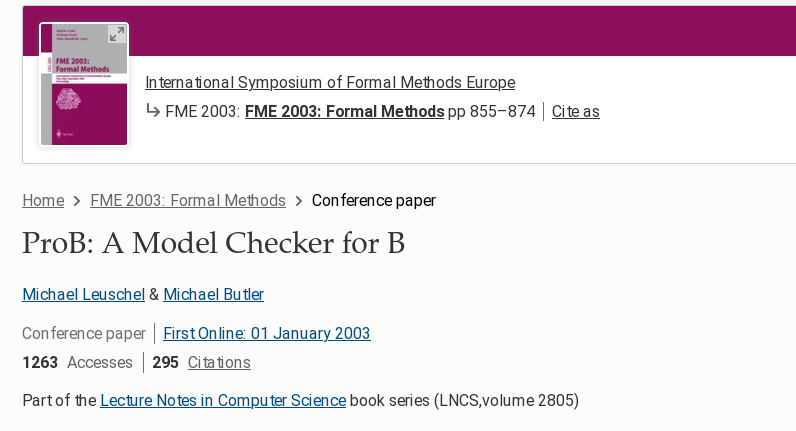
\includegraphics[scale=.5]{fig/prob-springer.png}
    \caption[Screenshot von \url{https://link.springer.com}]{
      Screenshot von \url{https://link.springer.com/chapter/10.1007/978-3-540-45236-2_46}}%
    \label{fig:prob-springer}
\end{figure}

Ein Beispiel ist der Artikel von Leuschel und Butler zu \textsc{ProB}~\cite{leuschel2003prob}.
In \cref{fig:prob-springer} sind die wichtigen Informationen für den Bibtex-Eintrag zu finden,
die Sie auf jeden Fall angeben sollten.
Ein Beispiel für einen passenden Bibtex-Eintrag lautet wie folgt (hier wird der \verb|InProceedings|-Typ verwendet):

\begin{verbatim}
@InProceedings(leuschel2003prob,
  Author	= {Leuschel, Michael and Butler, Michael},
  Title		= {{ProB}: A Model Checker for {B}},
  Year		= 2003,
  Month		= sep,
  Booktitle	= {{FME} 2003: Formal Methods},
  Series	= {LNCS},
  Volume	= 2805,
  Pages		= {855--874},
  Publisher	= {Springer},
  Address	= {Berlin, Heidelberg}
)
\end{verbatim}

\paragraph{Title, Author, Pages.} Diese Einträge sollten selbsterklärend sein.
\paragraph{Booktitle.} Hier gibt es mehrere valide Möglichkeiten.
Auf dem Buch selbst steht \enquote{FME 2003: Formal Methods}.
Akzeptabel wären auch \enquote{Proceedings FME 2003},
\enquote{Proceedings Formal Methods Europe (2003)},
\enquote{International Symposium of Formal Methods Europe. Pisa Italy, September 8-14, 2003, Proceedings}
oder Mischformen.
Wichtig ist, dass erkenntlich ist, zu welcher Konferenz aus welchem Jahr der Tagungsband stammt.
\paragraph{Year.} Leider erscheinen die Proceedings nicht unbedingt im selben Jahr wie die Konferenz selbst.
Daher ist auch das Jahr der Veröffentlichung anzugeben.
\paragraph{Series und Volume}. Proceedings vom Springer-Verlag erscheinen in der Regel in einer Reihe.
Üblich sind die LNCS (Lecture Notes in Computer Science). Darin erhalten sie auch eine Nummer, um sie eindeutig zu identifizieren.
Es gibt aber auch andere Reihen (z.B. LNAI oder CCIS); manchmal werden Tagungsbände auch mehreren Reihen zugeordnet.
Andere Herausgeber haben keine solche Reihe --- dann fallen diese Einträge weg.
\paragraph{Publisher.} Der Herausgeber der Proceedings.
Die meisten Tagungsbände werden vom Springer-Verlag oder der ACM veröffentlicht.
Hier gibt es auch mehrere valide Angaben (z.B. \enquote{Springer} bzw. \enquote{Springer-Verlag} oder \enquote{ACM} bzw. \enquote{Association for Computing Machinery}).
Diese sollten in Ihrer Bibliographie einheitlich sein.



\subsection{Sammelbände}

Es gibt einige Sammlungen an Artikeln, die als thematisches Buch veröffentlicht werden,
allerdings nicht aus einer Konferenz entstehen.
Ein Beispiel ist die Festschrift zu Egon Börgers 75.\ Geburtstag.
Darin findet man unter anderem den folgenden Artikel:

\begin{verbatim}
@InCollection(Leuschel2021,
  Author    = {Leuschel, Michael},
  Title     = {Spot the Difference: A Detailed Comparison Between {B}
                and Event-{B}},
  Booktitle = {Logic, Computation and Rigorous Methods},
  Publisher = {Springer},
  Year      = 2021,
  Volume    = 12750,
  Series    = {Lecture Notes in Computer Science},
  Pages     = {147--172}
)
\end{verbatim}

Insgesamt ist dies sehr ähnlich zum Konferenzartikel; deshalb wird her nicht näher auf die einzelnen Schlüssel eingegangen.
Auch dieses Buch wurde in der LNCS-Reihe veröffentlicht.

\subsection{Journal-Artikel}

Artikel in Journals werden in der Regel als hochwertiger als Konferenz-Artikel angesehen
und sind daher als Quelle zu bevorzugen.
Hier ist die Zeit für die Gutachten in der Regel länger und es wird genauer hingesehen.
Häufig entstehen Journal-Artikel aus Konferenzartikeln und sind ausführlichere Versionen.
Manchmal wird aber auch ohne eine Konferenz-Version direkt in einem Journal eingereicht.

Für die Bibliographie werden viele ähnliche Einträge wie beim Konferenzartikel verwendet,
allerdings ist der Typ hier \verb|Article|.

\begin{verbatim}
@Article(leuschel2008prob,
  Author	= {Leuschel, Michael and Butler, Michael},
  Title		= {{ProB}: An Automated Analysis Toolset for the {B} Method},
  Year		= 2008,
  Month		= mar,
  Journal	= {International Journal on Software Tools for
             Technology Transfer},
  Volume	= 10,
  Pages		= {185--203},
  Number	= 2
)
\end{verbatim}

\paragraph{Title, Author, Pages, Year.} Diese Einträge sollten wieder selbsterklärend sein.
\paragraph{Journal.} Die Artikel werden in einem Journal veröffentlicht, das einen Namen hat.
Hier gibt es in der Regel auch etablierte Abkürzungen (wie etwa \enquote{STTT} für
\enquote{International Journal on Software Tools for Technology Transfer}).
Das Format sollte hier auch einheitlich sein.
\paragraph{Volume und Number.} Journal-Artikel werden meist gesammelt periodisch veröffentlicht.
In der Regel wird die Volume-Zahl pro Jahr erhöht;
innerhalb einer Volume gibt es dann häufig mehrere Veröffentlichungen, die mit der \enquote{issue number} hochgezählt werden.
Wird das Journal also vierteljährlich veröffentlicht, geht der Number-Eintrag bis 4 hoch.
Manchmal gibt es auch \enquote{special issues} zu einem bestimmten Thema oder als Sammlung an Artikeln,
die aus einer bestimmten Konferenz hervorgingen.

\subsection{Monographien}

Einige Bücher werden von vollständig von wenigen Autoren geschrieben.
Hier werden insgesamt recht wenig Informationen benötigt,
wie etwa in dem Beispiel hier:

\begin{verbatim}
@Book(abrial1996b,
  Author	= {Abrial, Jean-Raymond},
  Title		= {The {B}-Book: Assigning Programs to Meanings},
  Year		= 1996,
  Publisher	= {Cambridge University Press},
  Address	= {New York, NY, USA}
)
\end{verbatim}

Leicht andere Arten der Monographien sind Abschlussarbeiten.
Hier haben Master- und Doktorarbeiten eigene Typen mit selbsterklärenden Schlüsseln.
Falls Sie eine Bachelorarbeit zitieren möchten, können Sie auch den Typen \verb|MastersThesis| verwenden.

\begin{verbatim}
@MastersThesis(eulynx_ma,
  Author    = {Abdul Rasheeq},
  Title     = {An Approach To Improve {SysML} Railway Specification
                Using {UML-B} And Event-{B}},
  School    = {Frankfurt University of Applied Sciences},
  Year      = 2019
)
\end{verbatim}

\begin{verbatim}
@PhDThesis(nummenmaa2013executable,
  Author    = {Nummenmaa, Timo},
  Title     = {Executable formal specifications in game development:
                Design, validation and evolution},
  School    = {University of Tampere},
  Year      = 2013
)
\end{verbatim}


%%%%%%%%%%%%%%%%%%%%%%%%%%%%%%%%%%%%%%%%%%%%%%%%%%%%%%%%%%%%%%%%%%%%%%%%%%%%%%%%
%% (Ende) Der Inhalt der Arbeit                                               %%
%%%%%%%%%%%%%%%%%%%%%%%%%%%%%%%%%%%%%%%%%%%%%%%%%%%%%%%%%%%%%%%%%%%%%%%%%%%%%%%%


\backmatter

\clearpage
\bibliography{references}
%% Depending on Language, use german alphadin or original alpha
\iflanguage{ngerman}{
  \bibliographystyle{alphadin}
}{
  \bibliographystyle{alpha}
}

\end{document}
